\documentclass[10pt,fleqn]{article} % Default font size and left-justified equations
\usepackage[%
    pdftitle={Informatique : Tris d'une liste de valeurs numériques},
    pdfauthor={Xavier Pessoles}]{hyperref}

%%%%%%%%%%%%%%%%%%%%%%%%%%%%%%%%%%%%%%%%%
% Original author:
% Mathias Legrand (legrand.mathias@gmail.com) with modifications by:
% Vel (vel@latextemplates.com)
% License:
% CC BY-NC-SA 3.0 (http://creativecommons.org/licenses/by-nc-sa/3.0/)
%%%%%%%%%%%%%%%%%%%%%%%%%%%%%%%%%%%%%%%%%

%----------------------------------------------------------------------------------------
%	VARIOUS REQUIRED PACKAGES AND CONFIGURATIONS
%----------------------------------------------------------------------------------------

\usepackage[top=2.5cm,bottom=2cm,left=2cm,right=2cm,headsep=40pt,a4paper]{geometry} % Page margins

\usepackage{graphicx} % Required for including pictures
\graphicspath{{images/}} % Specifies the directory where pictures are stored

\usepackage{lipsum} % Inserts dummy text

\usepackage{tikz} % Required for drawing custom shapes

\usepackage[french]{babel} % English language/hyphenation
\frenchbsetup{StandardLists=true} % Pour éviter la collision babel enumitem pour les listes

\usepackage{enumitem} % Customize lists
\setlist{nolistsep} % Reduce spacing between bullet points and numbered lists

\usepackage{booktabs} % Required for nicer horizontal rules in tables

\usepackage{xcolor} % Required for specifying colors by name
%\definecolor{ocre}{RGB}{243,102,25} % Define the orange color used for highlighting throughout the book
 \definecolor{ocre}{RGB}{49,133,156} % Couleur ''bleue''
\definecolor{violetf}{RGB}{112,48,160} % Couleur ''violet''
\usepackage{enumitem}
\usepackage{pifont} % Pour les dinglist
\usepackage{multicol}
\usepackage{array} % Centrage vertical dans les tableaux

%----------------------------------------------------------------------------------------
%	FONTS
%----------------------------------------------------------------------------------------

\usepackage{avant} % Use the Avantgarde font for headings
%\usepackage{times} % Use the Times font for headings
%\usepackage{mathptmx} % Use the Adobe Times Roman as the default text font together with math symbols from the Sym­bol, Chancery and Com­puter Modern fonts
\usepackage[adobe-utopia]{mathdesign}
\usepackage{microtype} % Slightly tweak font spacing for aesthetics
\usepackage[utf8]{inputenc} % Required for including letters with accents
\usepackage[T1]{fontenc} % Use 8-bit encoding that has 256 glyphs

%----------------------------------------------------------------------------------------
%	BIBLIOGRAPHY AND INDEX
%----------------------------------------------------------------------------------------

\usepackage[style=alphabetic,citestyle=numeric,sorting=nyt,sortcites=true,autopunct=true,babel=hyphen,hyperref=true,abbreviate=false,backref=true,backend=biber]{biblatex}
\addbibresource{bibliography.bib} % BibTeX bibliography file
\defbibheading{bibempty}{}

\usepackage{calc} % For simpler calculation - used for spacing the index letter headings correctly
\usepackage{makeidx} % Required to make an index
\makeindex % Tells LaTeX to create the files required for indexing

%----------------------------------------------------------------------------------------
%	MAIN TABLE OF CONTENTS
%----------------------------------------------------------------------------------------

\usepackage{titletoc} % Required for manipulating the table of contents

\setcounter{tocdepth}{2}     % Dans la table des matieres
\setcounter{secnumdepth}{2}

\contentsmargin{0cm} % Removes the default margin

% Part text styling
\titlecontents{part}[0cm]
{\addvspace{20pt}\centering\large\bfseries}
{}
{}
{}

% Chapter text styling
\titlecontents{chapter}[1.25cm] % Indentation
{\addvspace{12pt}\large\sffamily\bfseries} % Spacing and font options for chapters
{\color{ocre!60}\contentslabel[\Large\thecontentslabel]{1.25cm}\color{ocre}} % Chapter number
{\color{ocre}}  
{\color{ocre!60}\normalsize\;\titlerule*[.5pc]{.}\;\thecontentspage} % Page number

% Section text styling
\titlecontents{section}[1.25cm] % Indentation
{\addvspace{3pt}\sffamily\bfseries} % Spacing and font options for sections
{\color{ocre!60}\contentslabel[\thecontentslabel]{1.25cm} \color{ocre}} % Section number
{\color{ocre}}
{\hfill\color{ocre!60}\thecontentspage} % Page number
[]

% Subsection text styling
\titlecontents{subsection}[1.25cm] % Indentation
{\addvspace{1pt}\sffamily\small} % Spacing and font options for subsections
{\contentslabel[\thecontentslabel]{1.25cm}} % Subsection number
{}
{\ \titlerule*[.5pc]{.}\;\thecontentspage} % Page number
[]

% List of figures
\titlecontents{figure}[0em]
{\addvspace{-5pt}\sffamily}
{\thecontentslabel\hspace*{1em}}
{}
{\ \titlerule*[.5pc]{.}\;\thecontentspage}
[]

% List of tables
\titlecontents{table}[0em]
{\addvspace{-5pt}\sffamily}
{\thecontentslabel\hspace*{1em}}
{}
{\ \titlerule*[.5pc]{.}\;\thecontentspage}
[]

%----------------------------------------------------------------------------------------
%	MINI TABLE OF CONTENTS IN PART HEADS
%----------------------------------------------------------------------------------------

% Chapter text styling
\titlecontents{lchapter}[0em] % Indenting
{\addvspace{15pt}\large\sffamily\bfseries} % Spacing and font options for chapters
{\color{ocre}\contentslabel[\Large\thecontentslabel]{1.25cm}\color{ocre}} % Chapter number
{}  
{\color{ocre}\normalsize\sffamily\bfseries\;\titlerule*[.5pc]{.}\;\thecontentspage} % Page number

% Section text styling
\titlecontents{lsection}[0em] % Indenting
{\sffamily\small} % Spacing and font options for sections
{\contentslabel[\thecontentslabel]{1.25cm}} % Section number
{}
{}

% Subsection text styling
\titlecontents{lsubsection}[.5em] % Indentation
{\normalfont\footnotesize\sffamily} % Font settings
{}
{}
{}

%----------------------------------------------------------------------------------------
%	PAGE HEADERS
%----------------------------------------------------------------------------------------

\usepackage{fancyhdr} % Required for header and footer configuration



\pagestyle{fancy}
 \renewcommand{\headrulewidth}{0pt}
 \fancyhead{}
 \fancyhead[L]{%
 \noindent\begin{minipage}[c]{2.6cm}%
 
\includegraphics[width=2cm]{png/logo_lycee.png}%
 \end{minipage}}

\fancyhead[C]{\rule{8cm}{.5pt}}

 \fancyhead[R]{%
 \noindent\begin{minipage}[c]{3cm}
 \begin{flushright}
 \footnotesize{\textit{\textsf{\xxtete}}}%
 \end{flushright}
 \end{minipage}
}


\fancyfoot[C]{\rule{12cm}{.5pt}}
\renewcommand{\footrulewidth}{0.2pt}
\fancyfoot[C]{\footnotesize{\bfseries \thepage}}
\fancyfoot[L]{ 
\begin{minipage}[c]{.2\linewidth}
\noindent\footnotesize{{\xxauteur}}
\end{minipage}}


\fancyfoot[R]{\footnotesize{\xxpied}
\ifthenelse{\isodd{\value{page}}}{
\begin{tikzpicture}[overlay]
\node[shape=rectangle, 
      rounded corners = .25 cm,
	  draw= ocre,
	  line width=2pt, 
	  fill = ocre!10,
	  minimum width  = 2.5cm,
	  minimum height = 3cm,] at (\xxposongletx,\xxposonglety) {};
\node at (\xxposonglettext,\xxposonglety) {\rotatebox{90}{\textbf{\large\color{ocre}{\xxonglet}}}};
%{};
\end{tikzpicture}}{}
}
%
%
%
% Removes the header from odd empty pages at the end of chapters
\makeatletter
\renewcommand{\cleardoublepage}{
\clearpage\ifodd\c@page\else
\hbox{}
\vspace*{\fill}
\thispagestyle{empty}
\newpage
\fi}

\fancypagestyle{plain}{%
\fancyhf{} % vide l’en-tête et le pied~de~page.
%\fancyfoot[C]{\bfseries \thepage} % numéro de la page en cours en gras
% et centré en pied~de~page.
\fancyfoot[R]{\footnotesize{\xxpied}}
\fancyfoot[C]{\rule{12cm}{.5pt}}
\renewcommand{\footrulewidth}{0.2pt}
\fancyfoot[C]{\footnotesize{\bfseries \thepage}}
\fancyfoot[L]{ 
\begin{minipage}[c]{.2\linewidth}
\noindent\footnotesize{{\xxauteur}}
\end{minipage}}}



%----------------------------------------------------------------------------------------
%	THEOREM STYLES
%----------------------------------------------------------------------------------------

% Conflit avec la police adobe
%\usepackage{amsmath,amsfonts,amssymb,amsthm} % For math equations, theorems, symbols, etc
\usepackage{amsmath,amsthm}

\newcommand{\intoo}[2]{\mathopen{]}#1\,;#2\mathclose{[}}
\newcommand{\ud}{\mathop{\mathrm{{}d}}\mathopen{}}
\newcommand{\intff}[2]{\mathopen{[}#1\,;#2\mathclose{]}}
%\newtheorem{notation}{Notation}[chapter]
\newtheorem{notation}{Notation}[section]

% Boxed/framed environments
\newtheoremstyle{ocrenumbox}% % Theorem style name
{0pt}% Space above
{0pt}% Space below
{\normalfont}% % Body font
{}% Indent amount
{\small\bf\sffamily\color{ocre}}% % Theorem head font
{\;}% Punctuation after theorem head
{0.25em}% Space after theorem head
{\small\sffamily\color{ocre}\thmname{#1}\nobreakspace\thmnumber%{\@ifnotempty{#1}{}\@upn{#2}}% Theorem text (e.g. Theorem 2.1)
\thmnote{\nobreakspace\the\thm@notefont\sffamily\bfseries\color{black}---\nobreakspace#3.}} % Optional theorem note
\renewcommand{\qedsymbol}{$\blacksquare$}% Optional qed square


% Boite pour les corriges
\newtheoremstyle{correctionbox}% % Theorem style name
{0pt}% Space above
{0pt}% Space below
{\normalfont}% % Body font
{}% Indent amount
{\small\bf\sffamily\color{violet}}% % Theorem head font
{\;}% Punctuation after theorem head
{0.25em}% Space after theorem head
{\small\sffamily\color{ocre}\thmname{#1}\nobreakspace\thmnumber%{\@ifnotempty{#1}{}\@upn{#2}}% Theorem text (e.g. Theorem 2.1)
\thmnote{\nobreakspace\the\thm@notefont\sffamily\bfseries\color{black}---\nobreakspace#3.}} % Optional theorem note
\renewcommand{\qedsymbol}{$\blacksquare$}% Optional qed square



\newtheoremstyle{blacknumex}% Theorem style name
{5pt}% Space above
{5pt}% Space below
{\normalfont}% Body font
{} % Indent amount
{\small\bf\sffamily}% Theorem head font
{\;}% Punctuation after theorem head
{0.25em}% Space after theorem head
{\small\sffamily{\tiny\ensuremath{\blacksquare}}\nobreakspace\thmname{#1}\nobreakspace\thmnumber%{\@ifnotempty{#1}{}\@upn{#2}}% Theorem text (e.g. Theorem 2.1)
\thmnote{\nobreakspace\the\thm@notefont\sffamily\bfseries---\nobreakspace#3.}}% Optional theorem note

\newtheoremstyle{blacknumbox} % Theorem style name
{0pt}% Space above
{0pt}% Space below
{\normalfont}% Body font
{}% Indent amount
{\small\bf\sffamily}% Theorem head font
{\;}% Punctuation after theorem head
{0.25em}% Space after theorem head
{\small\sffamily\thmname{#1}\nobreakspace 
\thmnote{\nobreakspace\the\thm@notefont\sffamily\bfseries---\nobreakspace#3.}}% Optional theorem note

% Non-boxed/non-framed environments
\newtheoremstyle{ocrenum}% % Theorem style name
{5pt}% Space above
{5pt}% Space below
{\normalfont}% % Body font
{}% Indent amount
{\small\bf\sffamily\color{ocre}}% % Theorem head font
{\;}% Punctuation after theorem head
{0.25em}% Space after theorem head
{\small\sffamily\color{ocre}\thmname{#1}\nobreakspace\thmnumber{\@ifnotempty{#1}{}\@upn{#2}}% Theorem text (e.g. Theorem 2.1)
\thmnote{\nobreakspace\the\thm@notefont\sffamily\bfseries\color{black}---\nobreakspace#3.}} % Optional theorem note
\renewcommand{\qedsymbol}{$\blacksquare$}% Optional qed square
\makeatother

% Environnement pour les titres de parties
\newtheoremstyle{partiebox} 
{0pt}% Space above
{0pt}% Space below
{\normalfont}% Body font
{}% Indent amount
{\small\bf\sffamily}% Theorem head font
{\;}% Punctuation after theorem head
{0.25em}% Space after theorem head




% Defines the theorem text style for each type of theorem to one of the three styles above
\newcounter{dummy} 
\numberwithin{dummy}{section}
\theoremstyle{ocrenumbox}
%\newtheorem{theoremeT}[dummy]{Théorème}
\newtheorem{theoremeT}[dummy]{Théorème}
\newtheorem{resultatT}[dummy]{Résultat}
\newtheorem{savoirT}[dummy]{Savoir}
\newtheorem{methodeT}[dummy]{Méthode}
\newtheorem{objectifT}[dummy]{Objectif}
%\newtheorem{problem}{Problem}[chapter]
\newtheorem{problem}{Problem}[section]
%\newtheorem{exerciseT}{Exercise}[chapter]
\newtheorem{exerciseT}{Exercice}[section]

\theoremstyle{blacknumex}
%\newtheorem{exampleT}{Example}[chapter]
\newtheorem{exempleT}{Exemple}[section]
\newtheorem{termT}{Terminal\\}[section]
\newtheorem{pyT}{Python\\}[section]
\newtheorem{sciT}{Scilab\\}[section]

\theoremstyle{blacknumbox}
%\newtheorem{vocabulary}{Vocabulary}[chapter]
\newtheorem{vocabulary}{Vocabulaire}[section]
%\newtheorem{definitionT}{Definition}[section]
\newtheorem{definitionT}{Définition}[section]
\newtheorem{demoT}{Démonstration}[section]
\newtheorem{corollaryT}[dummy]{Corollaire}
\newtheorem{hypoT}{Hypothèse(s)}

\theoremstyle{ocrenum}
\newtheorem{proposition}[dummy]{Proposition}

\theoremstyle{partiebox}
\newtheorem{titrepartieT}[]{}
\newtheorem{titrechapitreT}[]{}

\theoremstyle{correctionbox}
\newtheorem{correctionT}[dummy]{\color{violet}{Correction}}

%----------------------------------------------------------------------------------------
%	DEFINITION OF COLORED BOXES
%----------------------------------------------------------------------------------------

\RequirePackage[framemethod=tikz]{mdframed} % Required for creating the theorem, definition, exercise and corollary boxes

% Theorem box
\newmdenv[skipabove=7pt,
skipbelow=7pt,
backgroundcolor=ocre!10,
linecolor=ocre,
innerleftmargin=5pt,
innerrightmargin=5pt,
innertopmargin=5pt,
leftmargin=0cm,
rightmargin=0cm,
innerbottommargin=5pt]{tBox}


% Correction
\newmdenv[skipabove=7pt,
skipbelow=7pt,
backgroundcolor=violet!10,
linecolor=violet,
innerleftmargin=5pt,
innerrightmargin=5pt,
innertopmargin=5pt,
leftmargin=0cm,
rightmargin=0cm,
innerbottommargin=5pt]{coBox}


% Exercise box	  
\newmdenv[skipabove=7pt,
skipbelow=7pt,
rightline=false,
leftline=true,
topline=false,
bottomline=false,
backgroundcolor=ocre!10,
linecolor=ocre,
innerleftmargin=5pt,
innerrightmargin=5pt,
innertopmargin=5pt,
innerbottommargin=5pt,
leftmargin=0cm,
rightmargin=0cm,
linewidth=4pt]{eBox}	

% Definition box
\newmdenv[skipabove=7pt,
skipbelow=7pt,
rightline=false,
leftline=true,
topline=false,
bottomline=false,
backgroundcolor=ocre!10,
linecolor=ocre,
innerleftmargin=5pt,
innerrightmargin=5pt,
innertopmargin=0pt,
leftmargin=0cm,
rightmargin=0cm,
linewidth=4pt,
innerbottommargin=0pt]{dBox}	

% Demonstration box
\newmdenv[skipabove=7pt,
skipbelow=7pt,
rightline=false,
leftline=true,
topline=false,
bottomline=false,
%backgroundcolor=ocre!10,
linecolor=ocre,
innerleftmargin=5pt,
innerrightmargin=5pt,
innertopmargin=0pt,
leftmargin=0cm,
rightmargin=0cm,
linewidth=4pt,
innerbottommargin=0pt]{demoBox}	

% Corollary box
\newmdenv[skipabove=7pt,
skipbelow=7pt,
rightline=false,
leftline=true,
topline=false,
bottomline=false,
linecolor=gray,
backgroundcolor=black!5,
innerleftmargin=5pt,
innerrightmargin=5pt,
innertopmargin=5pt,
leftmargin=0cm,
rightmargin=0cm,
linewidth=4pt,
innerbottommargin=5pt]{cBox}


% Hypothèses
\newmdenv[skipabove=7pt,
skipbelow=7pt,
rightline=false,
leftline=true,
topline=false,
bottomline=false,
linecolor=gray,
backgroundcolor=black!5,
innerleftmargin=5pt,
innerrightmargin=5pt,
innertopmargin=5pt,
leftmargin=0cm,
rightmargin=0cm,
linewidth=4pt,
innerbottommargin=5pt]{hyBox}


% Boite pour le titre de la partie (pBox)
\newmdenv[skipabove=7pt,
skipbelow=7pt,
rightline=true,
leftline=false,
topline=false,
bottomline=false,
linecolor=ocre,
backgroundcolor=none,
innerleftmargin=5pt,
innerrightmargin=5pt,
innertopmargin=5pt,
leftmargin=0cm,
rightmargin=0cm,
linewidth=4pt,
innerbottommargin=5pt]{pBox}

% Boite pour le titre du chapitre (chBox)
\newmdenv[skipabove=7pt,
skipbelow=7pt,
rightline=false,
leftline=true,
topline=false,
bottomline=false,
linecolor=ocre,
%backgroundcolor=black!5,
innerleftmargin=5pt,
innerrightmargin=5pt,
innertopmargin=5pt,
leftmargin=0cm,
rightmargin=0cm,
linewidth=4pt,
innerbottommargin=5pt]{chBox}


% Boite pour les exemples
\newmdenv[skipabove=7pt,
skipbelow=7pt,
rightline=false,
leftline=true,
topline=false,
bottomline=false,
linecolor=gray,
backgroundcolor=white,
innerleftmargin=5pt,
innerrightmargin=5pt,
innertopmargin=5pt,
leftmargin=0cm,
rightmargin=0cm,
linewidth=4pt,
innerbottommargin=5pt]{exBox}

% Boite pour le terminal
\newmdenv[skipabove=7pt,
skipbelow=7pt,
rightline=false,
leftline=true,
topline=false,
bottomline=false,
linecolor=gray,
backgroundcolor=white,
innerleftmargin=5pt,
innerrightmargin=5pt,
innertopmargin=5pt,
leftmargin=0cm,
rightmargin=0cm,
linewidth=4pt,
innerbottommargin=5pt]{termBox}


% Boite pour Python
\newmdenv[skipabove=7pt,
skipbelow=7pt,
rightline=false,
leftline=true,
topline=false,
bottomline=false,
linecolor=gray,
backgroundcolor=white,
innerleftmargin=5pt,
innerrightmargin=5pt,
innertopmargin=5pt,
leftmargin=0cm,
rightmargin=0cm,
linewidth=4pt,
innerbottommargin=5pt]{pyBox}

% Boite pour scilab
\newmdenv[skipabove=7pt,
skipbelow=7pt,
rightline=false,
leftline=true,
topline=false,
bottomline=false,
linecolor=gray,
backgroundcolor=white,
innerleftmargin=5pt,
innerrightmargin=5pt,
innertopmargin=5pt,
leftmargin=0cm,
rightmargin=0cm,
linewidth=4pt,
innerbottommargin=5pt]{sciBox}
% Creates an environment for each type of theorem and assigns it a theorem text style from the "Theorem Styles" section above and a colored box from above
\newenvironment{theorem}{\begin{tBox}\begin{theoremeT}}{\end{theoremeT}\end{tBox}}
\newenvironment{resultat}{\begin{tBox}\begin{resultatT}}{\end{resultatT}\end{tBox}}
\newenvironment{methode}{\begin{tBox}\begin{methodeT}}{\end{methodeT}\end{tBox}}
\newenvironment{savoir}{\begin{tBox}\begin{savoirT}}{\end{savoirT}\end{tBox}}
\newenvironment{obj}{\begin{tBox}\begin{objectifT}}{\end{objectifT}\end{tBox}}
\newenvironment{corrige}{\begin{coBox}\begin{correctionT}}{\end{correctionT}\end{coBox}}
\newenvironment{exercise}{\begin{eBox}\begin{exerciseT}}{\hfill{\color{ocre}\tiny\ensuremath{\blacksquare}}\end{exerciseT}\end{eBox}}				  
\newenvironment{exercice}{\begin{eBox}\begin{exerciseT}}{\hfill{\color{ocre}\tiny\ensuremath{\blacksquare}}\end{exerciseT}\end{eBox}}				  

\newenvironment{definition}{\begin{dBox}\begin{definitionT}}{\end{definitionT}\end{dBox}}	
\newenvironment{defi}{\begin{dBox}\begin{definitionT}}{\end{definitionT}\end{dBox}}	
\newenvironment{demo}{\begin{demoBox}\begin{demoT}}{\end{demoT}\end{demoBox}}	
%\newenvironment{exemple}{\begin{exempleT}}{\hfill{\tiny\ensuremath{\blacksquare}}\end{exempleT}}		
\newenvironment{corollary}{\begin{cBox}\begin{corollaryT}}{\end{corollaryT}\end{cBox}}
\newenvironment{hypo}{\begin{hyBox}\begin{hypoT}}{\end{hypoT}\end{hyBox}}	\newenvironment{exemple}{\begin{exBox}\begin{exempleT}}{\hfill{\tiny\ensuremath{\blacksquare}}\end{exempleT}\end{exBox}}	
\newenvironment{titrepartie}{\begin{pBox}\begin{titrepartieT}}{\end{titrepartieT}\end{pBox}}	
\newenvironment{titrechapitre}{\begin{chBox}\begin{titrechapitreT}}{\end{titrechapitreT}\end{chBox}}	

\newenvironment{term}{ \begin{termBox}\begin{termT}}{\end{termT}\end{termBox}}
\newenvironment{py}{ \begin{pyBox}\begin{pyT}}{\end{pyT}\end{pyBox}}
\newenvironment{sci}{ \begin{sciBox}\begin{sciT}}{\end{sciT}\end{sciBox}}

%----------------------------------------------------------------------------------------
%	REMARK ENVIRONMENT
%----------------------------------------------------------------------------------------

\newenvironment{remark}{\par\vspace{10pt}\small % Vertical white space above the remark and smaller font size
\begin{list}{}{
\leftmargin=35pt % Indentation on the left
\rightmargin=25pt}\item\ignorespaces % Indentation on the right
\makebox[-2.5pt]{\begin{tikzpicture}[overlay]
\node[draw=ocre!60,line width=1pt,circle,fill=ocre!25,font=\sffamily\bfseries,inner sep=2pt,outer sep=0pt] at (-15pt,0pt){\textcolor{ocre}{R}};\end{tikzpicture}} % Orange R in a circle
\advance\baselineskip -1pt}{\end{list}\vskip5pt} % Tighter line spacing and white space after remark

\newenvironment{rem}{\par\vspace{10pt}\small % Vertical white space above the remark and smaller font size
\begin{list}{}{
\leftmargin=35pt % Indentation on the left
\rightmargin=25pt}\item\ignorespaces % Indentation on the right
\makebox[-2.5pt]{\begin{tikzpicture}[overlay]
\node[draw=ocre!60,line width=1pt,circle,fill=ocre!25,font=\sffamily\bfseries,inner sep=2pt,outer sep=0pt] at (-15pt,0pt){\textcolor{ocre}{R}};\end{tikzpicture}} % Orange R in a circle
\advance\baselineskip -1pt}{\end{list}\vskip5pt} % Tighter line spacing and white space after remark


\newenvironment{warn}{\par\vspace{10pt}\small % Vertical white space above the remark and smaller font size
\begin{list}{}{
\leftmargin=35pt % Indentation on the left
\rightmargin=25pt}\item\ignorespaces % Indentation on the right
\makebox[-2.5pt]{\begin{tikzpicture}[overlay]
\node[draw=red!60,line width=1pt,circle,fill=red!25,font=\sffamily\bfseries,inner sep=2pt,outer sep=0pt] at (-15pt,0pt){\textcolor{black}{!}};\end{tikzpicture}} % Point d'exclamation dans un cercle
\advance\baselineskip -1pt}{\end{list}\vskip5pt} % Tighter line spacing and white space after remark


%----------------------------------------------------------------------------------------
%	SECTION NUMBERING IN THE MARGIN
%----------------------------------------------------------------------------------------

\makeatletter
\renewcommand{\@seccntformat}[1]{\llap{\textcolor{ocre}{\csname the#1\endcsname}\hspace{1em}}}                    
\renewcommand{\section}{\@startsection{section}{1}{\z@}
{-4ex \@plus -1ex \@minus -.4ex}
{1ex \@plus.2ex }
{\normalfont\large\sffamily\bfseries}}
\renewcommand{\subsection}{\@startsection {subsection}{2}{\z@}
{-3ex \@plus -0.1ex \@minus -.4ex}
{0.5ex \@plus.2ex }
{\normalfont\sffamily\bfseries}}
\renewcommand{\subsubsection}{\@startsection {subsubsection}{3}{\z@}
{-2ex \@plus -0.1ex \@minus -.2ex}
{.2ex \@plus.2ex }
{\normalfont\small\sffamily\bfseries}}                        
\renewcommand\paragraph{\@startsection{paragraph}{4}{\z@}
{-2ex \@plus-.2ex \@minus .2ex}
{.1ex}
{\normalfont\small\sffamily\bfseries}}

%----------------------------------------------------------------------------------------
%	PART HEADINGS
%----------------------------------------------------------------------------------------


%----------------------------------------------------------------------------------------
%	CHAPTER HEADINGS
%----------------------------------------------------------------------------------------

% \newcommand{\thechapterimage}{}%
% \newcommand{\chapterimage}[1]{\renewcommand{\thechapterimage}{#1}}%
% \def\@makechapterhead#1{%
% {\parindent \z@ \raggedright \normalfont
% \ifnum \c@secnumdepth >\m@ne
% \if@mainmatter
% \begin{tikzpicture}[remember picture,overlay]
% \node at (current page.north west)
% {\begin{tikzpicture}[remember picture,overlay]
% \node[anchor=north west,inner sep=0pt] at (0,0) {\includegraphics[width=\paperwidth]{\thechapterimage}};
% \draw[anchor=west] (\Gm@lmargin,-9cm) node [line width=2pt,rounded corners=15pt,draw=ocre,fill=white,fill opacity=0.5,inner sep=15pt]{\strut\makebox[22cm]{}};
% \draw[anchor=west] (\Gm@lmargin+.3cm,-9cm) node {\huge\sffamily\bfseries\color{black}\thechapter. #1\strut};
% \end{tikzpicture}};
% \end{tikzpicture}
% \else
% \begin{tikzpicture}[remember picture,overlay]
% \node at (current page.north west)
% {\begin{tikzpicture}[remember picture,overlay]
% \node[anchor=north west,inner sep=0pt] at (0,0) {\includegraphics[width=\paperwidth]{\thechapterimage}};
% \draw[anchor=west] (\Gm@lmargin,-9cm) node [line width=2pt,rounded corners=15pt,draw=ocre,fill=white,fill opacity=0.5,inner sep=15pt]{\strut\makebox[22cm]{}};
% \draw[anchor=west] (\Gm@lmargin+.3cm,-9cm) node {\huge\sffamily\bfseries\color{black}#1\strut};
% \end{tikzpicture}};
% \end{tikzpicture}
% \fi\fi\par\vspace*{270\p@}}}

%-------------------------------------------

\def\@makeschapterhead#1{%
\begin{tikzpicture}[remember picture,overlay]
\node at (current page.north west)
{\begin{tikzpicture}[remember picture,overlay]
\node[anchor=north west,inner sep=0pt] at (0,0) {\includegraphics[width=\paperwidth]{\thechapterimage}};
\draw[anchor=west] (\Gm@lmargin,-9cm) node [line width=2pt,rounded corners=15pt,draw=ocre,fill=white,fill opacity=0.5,inner sep=15pt]{\strut\makebox[22cm]{}};
\draw[anchor=west] (\Gm@lmargin+.3cm,-9cm) node {\huge\sffamily\bfseries\color{black}#1\strut};
\end{tikzpicture}};
\end{tikzpicture}
\par\vspace*{270\p@}}
\makeatother

%----------------------------------------------------------------------------------------
%	HYPERLINKS IN THE DOCUMENTS
%----------------------------------------------------------------------------------------


\hypersetup{hidelinks,backref=true,pagebackref=true,hyperindex=true,colorlinks=false,breaklinks=true,urlcolor= ocre,bookmarks=true,bookmarksopen=false,pdftitle={Title},pdfauthor={Author}}
\usepackage{bookmark}
\bookmarksetup{
open,
numbered,
addtohook={%
\ifnum\bookmarkget{level}=0 % chapter
\bookmarksetup{bold}%
\fi
\ifnum\bookmarkget{level}=-1 % part
\bookmarksetup{color=ocre,bold}%
\fi
}
}

%----------------------------------------------------------------------------------------
%	
%----------------------------------------------------------------------------------------

\newcommand{\thechapterimage}{}%
\newcommand{\chapterimage}[1]{\renewcommand{\thechapterimage}{#1}}%
\def\@makechapterhead#1{%
{\parindent \z@ \raggedright \normalfont
\begin{tikzpicture}[remember picture,overlay]
\node at (current page.north west)
{\begin{tikzpicture}[remember picture,overlay]
\node[anchor=north west,inner sep=0pt] at (0,0) {\includegraphics[width=\paperwidth]{\thechapterimage}};
%\draw[anchor=west] (\Gm@lmargin,-9cm) node [line width=2pt,rounded corners=15pt,draw=ocre,fill=white,fill opacity=0.5,inner sep=15pt]{\strut\makebox[22cm]{}};
%\draw[anchor=west] (\Gm@lmargin+.3cm,-9cm) node {\huge\sffamily\bfseries\color{black}\thechapter. #1\strut};
\end{tikzpicture}};
\end{tikzpicture}
\par\vspace*{270\p@}
}}




\makeatletter             
\renewcommand{\subparagraph}{\@startsection{subparagraph}{5}{\z@}%
                                    {-2ex \@plus-.2ex \@minus .2ex}%
                                    {0ex}%               
{\normalfont\bfseries Question \hspace{.7cm} }}
\makeatother
\renewcommand{\thesubparagraph}{\arabic{subparagraph}} 
\makeatletter


%%%% Environnement pour inclure du code
\usepackage{listings}
\lstloadlanguages{R}   % pour regler les pb d accent utf8 dans les codes
\lstset{language=R} % pour regler les pb d accent utf8 dans les codes
\renewcommand{\lstlistlistingname}{Listings}
\renewcommand{\lstlistingname}{Listing}

\definecolor{Bleu}{rgb}{0.1,0.1,1.0}
\definecolor{Noir}{rgb}{0,0,0}
\definecolor{Grau}{rgb}{0.5,0.5,0.5}
\definecolor{DunkelGrau}{rgb}{0.15,0.15,0.15}
\definecolor{Hellbraun}{rgb}{0.5,0.25,0.0}
\definecolor{Magenta}{rgb}{1.0,0.0,1.0}
\definecolor{Gris}{gray}{0.5}
\definecolor{Vert}{rgb}{0,0.5,0}
\definecolor{SourceHintergrund}{rgb}{1,1.0,0.95}


\lstnewenvironment{python}[1][]{
\lstset{
%escapeinside={\%*}{*)},
inputencoding=utf8,   % pour regler les pb d accent utf8 dans les codes
extendedchars=true,   % pour regler les pb d accent utf8 dans les codes
language=python,
basicstyle=\sffamily\footnotesize, 	
stringstyle=\color{red}, 
showstringspaces=false, 
alsoletter={1234567890},
otherkeywords={\ , \}, \{},
keywordstyle=\color{blue},
emph={access,and,break,class,continue,def,del,elif ,else,
except,exec,finally,for,from,global,if,import,in,i s,
lambda,not,or,pass,print,raise,return,try,while},
emphstyle=\color{black}\bfseries,
emph={[2]True, False, None, self},
emphstyle=[2]\color{black},
emph={[3]from, import, as},
emphstyle=[3]\color{blue},
upquote=true,
columns=flexible, % pour empecher d'avoir un espacement mono
morecomment=[s]{"""}{"""},
commentstyle=\color{Hellbraun}\slshape, 
%emph={[4]1, 2, 3, 4, 5, 6, 7, 8, 9, 0},
emphstyle=[4]\color{blue},
literate=*{:}{{\textcolor{blue}:}}{1}
{=}{{\textcolor{blue}=}}{1}
{-}{{\textcolor{blue}-}}{1}
{+}{{\textcolor{blue}+}}{1}
{*}{{\textcolor{blue}*}}{1}
{!}{{\textcolor{blue}!}}{1}
{(}{{\textcolor{blue}(}}{1}
{)}{{\textcolor{blue})}}{1}
{[}{{\textcolor{blue}[}}{1}
{]}{{\textcolor{blue}]}}{1}
{<}{{\textcolor{blue}<}}{1}
{>}{{\textcolor{blue}>}}{1}
{COMPLETER}{{\textcolor{red}COMPLETER}}{1},
literate=%
            {é}{{\'{e}}}1
            {è}{{\`{e}}}1
            {ê}{{\^{e}}}1
            {ë}{{\¨{e}}}1
            {û}{{\^{u}}}1
            {ù}{{\`{u}}}1
            {â}{{\^{a}}}1
            {à}{{\`{a}}}1
            {î}{{\^{i}}}1
            {ç}{{\c{c}}}1
            {Ç}{{\c{C}}}1
            {É}{{\'{E}}}1
            {Ê}{{\^{E}}}1
            {À}{{\`{A}}}1
            {Â}{{\^{A}}}1
            {Î}{{\^{I}}}1, % pour regler les pb d accent utf8 dans les codes
%framexleftmargin=1mm, framextopmargin=1mm, frame=shadowbox, rulesepcolor=\color{blue},#1
%backgroundcolor=\color{SourceHintergrund}, 
%framexleftmargin=1mm, framexrightmargin=1mm, framextopmargin=1mm, frame=single, framerule=1pt, rulecolor=\color{black},#1
}}{}



\lstnewenvironment{scilab}[1][]{
\lstset{
language=scilab,
basicstyle=\sffamily\footnotesize, 	
stringstyle=\color{red}, 
showstringspaces=false, 
alsoletter={1234567890},
otherkeywords={\ , \}, \{},
keywordstyle=\color{blue},
emph={access,and,break,class,continue,def,del,elif ,else,
except,exec,finally,for,from,global,if,import,in,i s,
lambda,not,or,pass,print,raise,return,try,while,Debut},
emphstyle=\color{black}\bfseries,
emph={[2]True, False, None, self},
emphstyle=[2]\color{black},
emph={[3]from, import, as},
emphstyle=[3]\color{blue},
upquote=true,
columns=flexible, % pour empecher d'avoir un espacement mono
morecomment=[s]{"""}{"""},
commentstyle=\color{Hellbraun}\slshape, 
%emph={[4]1, 2, 3, 4, 5, 6, 7, 8, 9, 0},
emphstyle=[4]\color{blue},
literate=*{:}{{\textcolor{blue}:}}{1}
{=}{{\textcolor{blue}=}}{1}
{-}{{\textcolor{blue}-}}{1}
{+}{{\textcolor{blue}+}}{1}
{*}{{\textcolor{blue}*}}{1}
{!}{{\textcolor{blue}!}}{1}
{(}{{\textcolor{blue}(}}{1}
{)}{{\textcolor{blue})}}{1}
{[}{{\textcolor{blue}[}}{1}
{]}{{\textcolor{blue}]}}{1}
{<}{{\textcolor{blue}<}}{1}
{>}{{\textcolor{blue}>}}{1},
%framexleftmargin=1mm, framextopmargin=1mm, frame=shadowbox, rulesepcolor=\color{blue},#1
%backgroundcolor=\color{SourceHintergrund}, 
%framexleftmargin=1mm, framexrightmargin=1mm, framextopmargin=1mm, frame=single, framerule=1pt, rulecolor=\color{black},#1
}}{}


\lstdefinestyle{stylepython}{%
escapeinside={\%*}{*)},
inputencoding=utf8,   % pour regler les pb d accent utf8 dans les codes
extendedchars=true,   % pour regler les pb d accent utf8 dans les codes
language=python,
basicstyle=\sffamily\footnotesize, 	
stringstyle=\color{red}, 
showstringspaces=false, 
alsoletter={1234567890},
otherkeywords={\ , \}, \{},
keywordstyle=\color{blue},
emph={access,and,break,class,continue,def,del,elif ,else,
except,exec,finally,for,from,global,if,import,in,i s,
lambda,not,or,pass,print,raise,return,try,while},
emphstyle=\color{black}\bfseries,
emph={[2]True, False, None, self},
emphstyle=[2]\color{green},
emph={[3]from, import, as},
emphstyle=[3]\color{blue},
upquote=true,
columns=flexible, % pour empecher d'avoir un espacement mono
morecomment=[s]{"""}{"""},
commentstyle=\color{Hellbraun}\slshape, 
%emph={[4]1, 2, 3, 4, 5, 6, 7, 8, 9, 0},
emphstyle=[4]\color{blue},
literate=*{:}{{\textcolor{blue}:}}{1}
{=}{{\textcolor{blue}=}}{1}
{-}{{\textcolor{blue}-}}{1}
{+}{{\textcolor{blue}+}}{1}
{*}{{\textcolor{blue}*}}{1}
{!}{{\textcolor{blue}!}}{1}
{(}{{\textcolor{blue}(}}{1}
{)}{{\textcolor{blue})}}{1}
{[}{{\textcolor{blue}[}}{1}
{]}{{\textcolor{blue}]}}{1}
{<}{{\textcolor{blue}<}}{1}
{>}{{\textcolor{blue}>}}{1}
{COMPLETER}{{\textcolor{red}COMPLETER}}{1},
literate=%
            {é}{{\'{e}}}1
            {è}{{\`{e}}}1
            {ê}{{\^{e}}}1
            {ë}{{\¨{e}}}1
            {û}{{\^{u}}}1
            {ù}{{\`{u}}}1
            {â}{{\^{a}}}1
            {à}{{\`{a}}}1
            {î}{{\^{i}}}1
            {ç}{{\c{c}}}1
            {Ç}{{\c{C}}}1
            {É}{{\'{E}}}1
            {Ê}{{\^{E}}}1
            {À}{{\`{A}}}1
            {Â}{{\^{A}}}1
            {Î}{{\^{I}}}1,
%numbers=left,                    % where to put the line-numbers; possible values are (none, left, right)
%numbersep=5pt,                   % how far the line-numbers are from the code
%numberstyle=\tiny\color{mygray}, % the style that is used for the line-numbers
}



\lstnewenvironment{termi}[1][]{
\lstset{
language=scilab,
basicstyle=\sffamily\footnotesize, 	
stringstyle=\color{red}, 
showstringspaces=false, 
alsoletter={1234567890},
otherkeywords={\ , \}, \{},
keywordstyle=\color{blue},
emph={access,and,break,class,continue,def,del,elif ,else,
except,exec,finally,for,from,global,if,import,in,i s,
lambda,not,or,pass,print,raise,return,try,while,Debut},
emphstyle=\color{black}\bfseries,
emph={[2]True, False, None, self},
emphstyle=[2]\color{green},
emph={[3]from, import, as},
emphstyle=[3]\color{blue},
upquote=true,
columns=flexible, % pour empecher d'avoir un espacement mono
morecomment=[s]{"""}{"""},
commentstyle=\color{Hellbraun}\slshape, 
%emph={[4]1, 2, 3, 4, 5, 6, 7, 8, 9, 0},
emphstyle=[4]\color{blue},
literate=*{:}{{\textcolor{blue}:}}{1}
{=}{{\textcolor{blue}=}}{1}
{-}{{\textcolor{blue}-}}{1}
{+}{{\textcolor{blue}+}}{1}
{*}{{\textcolor{blue}*}}{1}
{!}{{\textcolor{blue}!}}{1}
{(}{{\textcolor{blue}(}}{1}
{)}{{\textcolor{blue})}}{1}
{[}{{\textcolor{blue}[}}{1}
{]}{{\textcolor{blue}]}}{1}
{<}{{\textcolor{blue}<}}{1}
{>}{{\textcolor{blue}>}}{1},
%framexleftmargin=1mm, framextopmargin=1mm, frame=shadowbox, rulesepcolor=\color{blue},#1
%backgroundcolor=\color{SourceHintergrund}, 
%framexleftmargin=1mm, framexrightmargin=1mm, framextopmargin=1mm, frame=single, framerule=1pt, rulecolor=\color{black},#1
}}{}


\lstnewenvironment{sql}[1][]{
\lstset{
%escapeinside={\%*}{*)},
%inputencoding=utf8,   % pour regler les pb d accent utf8 dans les codes
%extendedchars=true,   % pour regler les pb d accent utf8 dans les codes
language=sql,
basicstyle=\sffamily\footnotesize, 	
stringstyle=\color{red}, 
showstringspaces=false, 
alsoletter={1234567890},
otherkeywords={\ , \}, \{},
keywordstyle=\color{blue},
emph={access,and,break,class,continue,def,del,elif ,else,
except,exec,finally,for,from,global,if,import,in,i s,
lambda,not,or,pass,print,raise,return,try,while},
emphstyle=\color{black}\bfseries,
emph={[2]True, False, None, self},
emphstyle=[2]\color{black},
emph={[3]from, import, as},
emphstyle=[3]\color{blue},
upquote=true,
columns=flexible, % pour empecher d'avoir un espacement mono
morecomment=[s]{"""}{"""},
commentstyle=\color{Hellbraun}\slshape, 
%emph={[4]1, 2, 3, 4, 5, 6, 7, 8, 9, 0},
emphstyle=[4]\color{blue},
literate=*{:}{{\textcolor{blue}:}}{1}
{=}{{\textcolor{blue}=}}{1}
{-}{{\textcolor{blue}-}}{1}
{+}{{\textcolor{blue}+}}{1}
{*}{{\textcolor{blue}*}}{1}
{!}{{\textcolor{blue}!}}{1}
{(}{{\textcolor{blue}(}}{1}
{)}{{\textcolor{blue})}}{1}
{[}{{\textcolor{blue}[}}{1}
{]}{{\textcolor{blue}]}}{1}
{<}{{\textcolor{blue}<}}{1}
{>}{{\textcolor{blue}>}}{1}
{COMPLETER}{{\textcolor{red}COMPLETER}}{1},
literate=%
            {é}{{\'{e}}}1
            {è}{{\`{e}}}1
            {ê}{{\^{e}}}1
            {ë}{{\¨{e}}}1
            {û}{{\^{u}}}1
            {ù}{{\`{u}}}1
            {â}{{\^{a}}}1
            {à}{{\`{a}}}1
            {î}{{\^{i}}}1
            {ç}{{\c{c}}}1
            {Ç}{{\c{C}}}1
            {É}{{\'{E}}}1
            {Ê}{{\^{E}}}1
            {À}{{\`{A}}}1
            {Â}{{\^{A}}}1
            {Î}{{\^{I}}}1, % pour regler les pb d accent utf8 dans les codes
%framexleftmargin=1mm, framextopmargin=1mm, frame=shadowbox, rulesepcolor=\color{blue},#1
%backgroundcolor=\color{SourceHintergrund}, 
%framexleftmargin=1mm, framexrightmargin=1mm, framextopmargin=1mm, frame=single, framerule=1pt, rulecolor=\color{black},#1
}}{}


% Définition des booleéns
\newif\iffiche
\newif\ifprof
\newif\iftd
\newif\ifcours

%%%%%%%%%%%%
% Définition des vecteurs 
%%%%%%%%%%%%
\newcommand{\vect}[1]{\overrightarrow{#1}}
\newcommand{\axe}[2]{\left(#1,\vect{#2}\right)}
\newcommand{\couple}[2]{\left(#1,\vect{#2}\right)}
\newcommand{\angl}[2]{\left(\vect{#1},\vect{#2}\right)}

\newcommand{\rep}[1]{\mathcal{R}_{#1}}
\newcommand{\quadruplet}[4]{\left(#1;#2,#3,#4 \right)}
\newcommand{\repere}[4]{\left(#1;\vect{#2},\vect{#3},\vect{#4} \right)}
\newcommand{\base}[3]{\left(\vect{#1},\vect{#2},\vect{#3} \right)}


\newcommand{\vx}[1]{\vect{x_{#1}}}
\newcommand{\vy}[1]{\vect{y_{#1}}}
\newcommand{\vz}[1]{\vect{z_{#1}}}

\newcommand{\norm}[1]{\ensuremath{\left\Vert {#1}\right\Vert}}
\newcommand{\Ker}{\mathop{\mathrm{Ker}}\nolimits}

% d droit pour le calcul différentiel
\newcommand{\dd}{\text{d}}

\newcommand{\inertie}[2]{I_{#1}\left( #2\right)}
\newcommand{\matinertie}[7]{
\begin{pmatrix}
#1 & #6 & #5 \\
#6 & #2 & #4 \\
#5 & #4 & #3 \\
\end{pmatrix}_{#7}}
%%%%%%%%%%%%
% Définition des torseurs 
%%%%%%%%%%%%

\newcommand{\ec}[2]{%
\mathcal{E}_c\left(#1/#2\right)}

\newcommand{\pext}[3]{%
\mathcal{P}\left(#1\rightarrow#2/#3\right)}

\newcommand{\pint}[3]{%
\mathcal{P}\left(#1 \stackrel{\text{#3}}{\leftrightarrow} #2\right)}


 \newcommand{\torseur}[1]{%
\left\{{#1}\right\}
}

\newcommand{\torseurcin}[3]{%
\left\{\mathcal{#1} \left(#2/#3 \right) \right\}
}

\newcommand{\torseurci}[2]{%
\left\{\sigma \left(#1/#2 \right) \right\}
}
\newcommand{\torseurdyn}[2]{%
\left\{\mathcal{D} \left(#1/#2 \right) \right\}
}


\newcommand{\torseurstat}[3]{%
\left\{\mathcal{#1} \left(#2\rightarrow #3 \right) \right\}
}


 \newcommand{\torseurc}[8]{%
%\left\{#1 \right\}=
\left\{
{#1}
\right\}
 = 
\left\{%
\begin{array}{cc}%
{#2} & {#5}\\%
{#3} & {#6}\\%
{#4} & {#7}\\%
\end{array}%
\right\}_{#8}%
}

 \newcommand{\torseurcol}[7]{
\left\{%
\begin{array}{cc}%
{#1} & {#4}\\%
{#2} & {#5}\\%
{#3} & {#6}\\%
\end{array}%
\right\}_{#7}%
}

 \newcommand{\torseurl}[3]{%
%\left\{\mathcal{#1}\right\}_{#2}=%
\left\{%
\begin{array}{l}%
{#1} \\%
{#2} %
\end{array}%
\right\}_{#3}%
}

% Vecteur vitesse
 \newcommand{\vectv}[3]{%
\vect{V\left( {#1} \in {#2}/{#3}\right)}
}

% Vecteur force
\newcommand{\vectf}[2]{%
\vect{R\left( {#1} \rightarrow {#2}\right)}
}

% Vecteur moment stat
\newcommand{\vectm}[3]{%
\vect{\mathcal{M}\left( {#1}, {#2} \rightarrow {#3}\right)}
}




% Vecteur résultante cin
\newcommand{\vectrc}[2]{%
\vect{R_c \left( {#1}/ {#2}\right)}
}
% Vecteur moment cin
\newcommand{\vectmc}[3]{%
\vect{\sigma \left( {#1}, {#2} /{#3}\right)}
}


% Vecteur résultante dyn
\newcommand{\vectrd}[2]{%
\vect{R_d \left( {#1}/ {#2}\right)}
}
% Vecteur moment dyn
\newcommand{\vectmd}[3]{%
\vect{\delta \left( {#1}, {#2} /{#3}\right)}
}

% Vecteur accélération
 \newcommand{\vectg}[3]{%
\vect{\Gamma \left( {#1} \in {#2}/{#3}\right)}
}

% Vecteur omega
 \newcommand{\vecto}[2]{%
\vect{\Omega\left( {#1}/{#2}\right)}
}
% }$$\left\{\mathcal{#1} \right\}_{#2} =%
% \left\{%
% \begin{array}{c}%
%  #3 \\%
%  #4 %
% \end{array}%
% \right\}_{#5}}

\newcommand{\N}{\mathbb{N}}
\newcommand{\Z}{\mathbb{Z}}
\newcommand{\R}{\mathbb{R}}
\newcommand{\C}{\mathbb{C}}
\newcommand{\K}{\mathbb{K}}

\newcommand{\cA}{\mathscr{A}}
\newcommand{\cM}{\mathscr{M}}
\newcommand{\cL}{\mathscr{L}}
\newcommand{\cS}{\mathscr{S}}

\newcommand{\python}{\texttt{Python}}

\newcommand{\z}[1]{\Z_{#1}}
\newcommand{\ztimes}[1]{\Z_{#1}^{\times}}
\newcommand{\ii}[1]{[\![#1[\![}
\newcommand{\iif}[1]{[\![#1]\!]}
\newcommand{\llbr}{\ensuremath{\llbracket}}
\newcommand{\rrbr}{\ensuremath{\rrbracket}}
%\newcommand{\p}[1]{\left(#1\right)}
\newcommand{\ens}[1]{\left\{ #1 \right\}}
\newcommand{\croch}[1]{\left[ #1 \right]}
%\newcommand{\of}[1]{\lstinline{#1}}
% \newcommand{\py}[2]{%
%   \begin{tabular}{|l}
%     \lstinline+>>>+\textbf{\of{#1}}\\
%     \of{#2}
%   \end{tabular}\par{}
% }
\newcommand{\floor}[1]{\left\lfloor#1\right\rfloor}
\newcommand{\ceil}[1]{\left\lceil#1\right\rceil}
\newcommand{\abs}[1]{\left|#1\right|}


% Binaire, octal, hexa
\newcommand{\hex}[1]{\underline{\text{\texttt{#1}}}_{16}}
\newcommand{\oct}[1]{\underline{\text{\texttt{#1}}}_{8}}
\newcommand{\bin}[1]{\underline{\text{\texttt{#1}}}_{2}}
\DeclareMathOperator{\mmod}{\texttt{\%}}


% Fonctions et systèmes
\newcommand{\fct}[5][t]{%
  \begin{array}[#1]{rcl}
    #2 & \rightarrow & #3\\
    #4 & \mapsto     & #5\\
  \end{array}
}
\newcommand{\fonction}[5]{#1 : \left\{\begin{array}{rcl} #2& \longrightarrow &#3 \\ #4 &\longmapsto & #5\end{array}\right.}
\newenvironment{systeme}{\left\{ \begin{array}{rcl}}{\end{array}\right.}

% Matrices
\newcommand{\mat}[1]{
  \begin{pmatrix}
    #1
  \end{pmatrix}
}
\newcommand{\inv}{\ensuremath{^{-1}}}
\newcommand{\bpm}{\begin{pmatrix}}
\newcommand{\epm}{\end{pmatrix}}


% bases de données
\newcommand{\relat}[1]{\textsc{#1}}
\newcommand{\attr}[1]{\emph{#1}}
\newcommand{\prim}[1]{\uline{#1}}
\newcommand{\foreign}[1]{\#\textsl{#1}}


% Bases de données

\newcommand{\att}{\ensuremath{\mathbf{att}}}
\newcommand{\dom}{\ensuremath{\mathbf{dom}}}
\newcommand{\sort}{\ensuremath{\mathbf{sort}}}
\newcommand{\relname}{\ensuremath{\mathbf{relname}}}
\newcommand{\var}{\ensuremath{\mathbf{var}}}
\newcommand{\FILM}{\ensuremath{\mathtt{FILM}}}
\newcommand{\JOUE}{\ensuremath{\mathtt{JOUE}}}
\newcommand{\PERSONNE}{\ensuremath{\mathtt{PERSONNE}}}
\newcommand{\PERSONNAGE}{\ensuremath{\mathtt{PERSONNAGE}}}

\newcommand{\ttid}{\ensuremath{\mathtt{id}}}
\newcommand{\tttitre}{\ensuremath{\mathtt{titre}}}
\newcommand{\ttdate}{\ensuremath{\mathtt{date}}}
\newcommand{\ttidr}{\ensuremath{\mathtt{idrealisateur}}}
\newcommand{\ttdatenais}{\ensuremath{\mathtt{datenaissance}}}
\newcommand{\ttnom}{\ensuremath{\mathtt{nom}}}
\newcommand{\ttprenom}{\ensuremath{\mathtt{prenom}}}
\newcommand{\ttidacteur}{\ensuremath{\mathtt{idacteur}}}
\newcommand{\ttidfilm}{\ensuremath{\mathtt{idfilm}}}
\newcommand{\ttidpersonnage}{\ensuremath{\mathtt{idpersonnage}}}

\newcommand{\fv}{\mathrm{libre}}
\newcommand{\sem}[1]{[\![ #1 ]\!]}

\usepackage{colortbl}
%\fichetrue
\fichefalse

%\proftrue
\proffalse

%\tdtrue
\tdfalse

\courstrue
%\coursfalse

% -------------------------------------
% Déclaration des titres
% -------------------------------------

\def\discipline{Informatique}
\def\xxtete{Informatique}
\def\classe{PT}
\def\xxnumpartie{Partie 5}
\def\xxpartie{Algorithmique \& Programmation (Suite)}

\def\xxnumchapitre{Chapitre 3}
\def\xxchapitre{\hspace{.12cm} Tri d'une liste de valeurs numériques}

\def\xxposongletx{2}
\def\xxposonglettext{1.45}
\def\xxposonglety{13}%10

\def\xxonglet{Part. 5 -- Ch. 3}

\def\xxactivite{Cours}
\def\xxauteur{\textsl{Patrick Beynet }}%\\ Xavier Pessoles}}

\def\xxcompetences{%
\textsl{%
\textbf{Savoirs et compétences :}
\begin{itemize}[label=\ding{112},font=\color{ocre}] 
\item Alg -- C17 : tris d’un tableau à une dimension de valeurs numériques (tri par insertion, tri rapide, tri fusion).
\end{itemize}
}}

\def\xxfigures{

\includegraphics[width=\textwidth]{images/cartes}
%\textit{Tour de Hanoi [2]}
}%figues de la page de garde

\def\xxpied{%
Partie 5 -- Algorithmique et Programmation\\
Ch 3 : Tri d'une liste de valeurs numériques -- \xxactivite%
}


\newcommand{\bfsf}[1]{\small\textbf{\texttt{#1}}}
\newcommand{\tsf}[1]{\small{\texttt{#1}}}
%---------------------------------------------------------------------------
\begin{document}
\chapterimage{png/Fond_ALG}
\pagestyle{empty}


%%%%%%%% PAGE DE GARDE COURS
\ifcours
\begin{tikzpicture}[remember picture,overlay]
\node at (current page.north west)
{\begin{tikzpicture}[remember picture,overlay]
\node[anchor=north west,inner sep=0pt] at (0,0) {\includegraphics[width=\paperwidth]{\thechapterimage}};
\draw[anchor=west] (-2cm,-8cm) node [line width=2pt,rounded corners=15pt,draw=ocre,fill=white,fill opacity=0.6,inner sep=40pt]{\strut\makebox[22cm]{}};
\draw[anchor=west] (1cm,-8cm) node {\huge\sffamily\bfseries\color{black} %
\begin{minipage}{1cm}
\rotatebox{90}{\LARGE\sffamily\textsc{\color{ocre}\textbf{\xxnumpartie}}}
\end{minipage} \hfill
\begin{minipage}[c]{14cm}
\begin{titrepartie}
\begin{flushright}
\renewcommand{\baselinestretch}{1.1} 
\Large\sffamily\textsc{\textbf{\xxpartie}}
\renewcommand{\baselinestretch}{1} 
\end{flushright}
\end{titrepartie}
\end{minipage} \hfill
\begin{minipage}[c]{3.5cm}
{\large\sffamily\textsc{\textbf{\color{ocre} \discipline}}}
\end{minipage} 
 };
\end{tikzpicture}};
\end{tikzpicture}


\begin{tikzpicture}[overlay]
\node[shape=rectangle, 
      rounded corners = .25 cm,
	  draw= ocre,
	  line width=2pt, 
	  fill = ocre!10,
	  minimum width  = 2.5cm,
	  minimum height = 3cm,] at (18cm,0) {};
\node at (17.7cm,0) {\rotatebox{90}{\textbf{\Large\color{ocre}{\classe}}}};
%{};
\end{tikzpicture}

\vspace{3.5cm}

\begin{tikzpicture}[remember picture,overlay]
\draw[anchor=west] (-2cm,-6cm) node {\huge\sffamily\bfseries\color{black} %
\begin{minipage}{2cm}
\begin{center}
\LARGE\sffamily\textsc{\color{ocre}\textbf{\xxactivite}}
\end{center}
\end{minipage} \hfill
\begin{minipage}[c]{15cm}
\begin{titrechapitre}
\renewcommand{\baselinestretch}{1.1} 
\Large\sffamily\textsc{\textbf{\xxnumchapitre}}

\Large\sffamily\textsc{\textbf{\xxchapitre}}
\vspace{.5cm}

\renewcommand{\baselinestretch}{1} 
\normalsize\normalfont
\xxcompetences
\end{titrechapitre}
\end{minipage}  };
\end{tikzpicture}
\vfill

\begin{flushright}
\begin{minipage}[c]{.3\linewidth}
\begin{center}
\xxfigures
\end{center}
\end{minipage}\hfill
\begin{minipage}[c]{.6\linewidth}
\startcontents
\printcontents{}{1}{}
\end{minipage}
\end{flushright}

\begin{tikzpicture}[remember picture,overlay]
\draw[anchor=west] (4.5cm,-.7cm) node {
\begin{minipage}[c]{.2\linewidth}
\begin{flushright}

\includegraphics[width=2cm]{png/logoCC}
\end{flushright}
\end{minipage}
\begin{minipage}[c]{.2\linewidth}
\textsl{\xxauteur} \\
\textsl{\classe}
\end{minipage}
 };
\end{tikzpicture}
\newpage
\pagestyle{fancy}

\newpage
\pagestyle{fancy}

\else
\fi


%%%%%%%% PAGE DE GARDE TD
\iftd
%\begin{tikzpicture}[remember picture,overlay]
%\node at (current page.north west)
%{\begin{tikzpicture}[remember picture,overlay]
%\draw[anchor=west] (-2cm,-3.25cm) node [line width=2pt,rounded corners=15pt,draw=ocre,fill=white,fill opacity=0.6,inner sep=40pt]{\strut\makebox[22cm]{}};
%\draw[anchor=west] (1cm,-3.25cm) node {\huge\sffamily\bfseries\color{black} %
%\begin{minipage}{1cm}
%\rotatebox{90}{\LARGE\sffamily\textsc{\color{ocre}\textbf{\xxnumpartie}}}
%\end{minipage} \hfill
%\begin{minipage}[c]{13.5cm}
%\begin{titrepartie}
%\begin{flushright}
%\renewcommand{\baselinestretch}{1.1} 
%\Large\sffamily\textsc{\textbf{\xxpartie}}
%\renewcommand{\baselinestretch}{1} 
%\end{flushright}
%\end{titrepartie}
%\end{minipage} \hfill
%\begin{minipage}[c]{3.5cm}
%{\large\sffamily\textsc{\textbf{\color{ocre} \discipline}}}
%\end{minipage} 
% };
%\end{tikzpicture}};
%\end{tikzpicture}

%%%%%%%%%% PAGE DE GARDE TD %%%%%%%%%%%%%%%
%\begin{tikzpicture}[overlay]
%\node[shape=rectangle, 
%      rounded corners = .25 cm,
%	  draw= ocre,
%	  line width=2pt, 
%	  fill = ocre!10,
%	  minimum width  = 2.5cm,
%	  minimum height = 2.5cm,] at (18.5cm,0) {};
%\node at (17.7cm,0) {\rotatebox{90}{\textbf{\Large\color{ocre}{\classe}}}};
%%{};
%\end{tikzpicture}

% PARTIE ET CHAPITRE
%\begin{tikzpicture}[remember picture,overlay]
%\draw[anchor=west] (-1cm,-2.1cm) node {\large\sffamily\bfseries\color{black} %
%\begin{minipage}[c]{15cm}
%\begin{flushleft}
%\xxnumchapitre \\
%\xxchapitre
%\end{flushleft}
%\end{minipage}  };
%\end{tikzpicture}

% Bandeau titre exo
\begin{tikzpicture}[remember picture,overlay]
\draw[anchor=west] (-2cm,-4cm) node {\huge\sffamily\bfseries\color{black} %
\begin{minipage}{5cm}
\begin{center}
\LARGE\sffamily\color{ocre}\textbf{\textsc{\xxactivite}}

\begin{center}
\xxfigures
\end{center}

\end{center}
\end{minipage} \hfill
\begin{minipage}[c]{12cm}
\begin{titrechapitre}
\renewcommand{\baselinestretch}{1.1} 
\large\sffamily\textbf{\textsc{\xxtitreexo}}

\small\sffamily{\textbf{\textit{\color{black!70}\xxsourceexo}}}
\vspace{.5cm}

\renewcommand{\baselinestretch}{1} 
\normalsize\normalfont
\xxcompetences
\end{titrechapitre}
\end{minipage}  };
\end{tikzpicture}
\else
\fi


%%%%%%%% PAGE DE GARDE FICHE
\iffiche
\begin{tikzpicture}[remember picture,overlay]
\node at (current page.north west)
{\begin{tikzpicture}[remember picture,overlay]
\draw[anchor=west] (-2cm,-3.25cm) node [line width=2pt,rounded corners=15pt,draw=ocre,fill=white,fill opacity=0.6,inner sep=40pt]{\strut\makebox[22cm]{}};
\draw[anchor=west] (1cm,-3.25cm) node {\huge\sffamily\bfseries\color{black} %
\begin{minipage}{1cm}
\rotatebox{90}{\LARGE\sffamily\textsc{\color{ocre}\textbf{\xxnumpartie}}}
\end{minipage} \hfill
\begin{minipage}[c]{14cm}
\begin{titrepartie}
\begin{flushright}
\renewcommand{\baselinestretch}{1.1} 
\large\sffamily\textsc{\textbf{\xxpartie} \\} 

\vspace{.2cm}

\normalsize\sffamily\textsc{\textbf{\xxnumchapitre -- \xxchapitre}}
\renewcommand{\baselinestretch}{1} 
\end{flushright}
\end{titrepartie}
\end{minipage} \hfill
\begin{minipage}[c]{3.5cm}
{\large\sffamily\textsc{\textbf{\color{ocre} \discipline}}}
\end{minipage} 
 };
\end{tikzpicture}};
\end{tikzpicture}


\begin{tikzpicture}[overlay]
\node[shape=rectangle, 
      rounded corners = .25 cm,
	  draw= ocre,
	  line width=2pt, 
	  fill = ocre!10,
	  minimum width  = 2.5cm,
	  minimum height = 2.5cm,] at (18.5cm,0.5cm) {};
%	  minimum height = 2.5cm,] at (18.5cm,0cm) {};
\node at (17.7cm,0.5) {\rotatebox{90}{\textsf{\textbf{\large\color{ocre}{\classe}}}}};
%{};
\end{tikzpicture}

\else
\fi



%---------------------------------------------------------------------------

\section{Présentation}
Un algorithme de tri est un algorithme qui permet d'organiser une collection d'objets selon un ordre déterminé. Le tri permet notamment de faciliter les recherches ultérieures d'un élément dans une liste (recherche dichotomique).
On s'intéresse ici à des méthodes de tri d'une liste de valeurs numériques. Celle-ci est implémentée sous la forme d'un tableau à une dimension.

\begin{rem}
Pour trier des chaînes de caractères (mots), il suffit d'associer une valeur numérique à chaque caractère (code ASCII par exemple). 
On se limite dans le cadre du programme aux cas détaillés du tri par insertion, du tri rapide et du tri fusion.
\end{rem}

\section{Tri par insertion}
\subsection{Exemple du tri de carte}

Soit un paquet de « $n$ » cartes. On prend la première dans une main.
On saisie la seconde carte et on l'insère avant ou après la première selon le cas.
A l'étape « $i$ », la ième carte est insérée à sa place dans le paquet déjà trié. 
Pour cela, on peut :
\begin{itemize}
\item soit partir du début du tas déjà trié et s'arrêter lorsqu'on rencontre une carte plus grande que la i\ieme (méthode 1);
\item soit partir de la fin du tas déjà trié, et s'arrêter si on rencontre une carte plus petite que la i\ieme (méthode 2).
\end{itemize}
Le paquet contient alors « $i$ » cartes triées. On procède ainsi de suite jusqu'à la dernière carte.

\subsection{Application à une liste de nombres}

\begin{tabular}{|c|c|c|c|c|}
\hline
5 & 8 & 3 & 2 & 9 \\
\hline
\end{tabular}

\begin{minipage}[b]{.07\linewidth}
Étape 1 
\end{minipage}\hfill
\begin{minipage}[b]{.15\linewidth}
\begin{tabular}{|c|c|c|c|c|}
\hline
\cellcolor{black!10}5 & \cellcolor{black!30}8 & 3 & 2 & 9 \\
\hline
\end{tabular}
\end{minipage}\hfill
\begin{minipage}[b]{.05\linewidth}
$$
\Longrightarrow
$$
\end{minipage}\hfill
\begin{minipage}[b]{.15\linewidth}
\begin{tabular}{|c|c|c|c|c|}
\hline
\cellcolor{black!10}5 & \cellcolor{black!30}8 & 3 & 2 & 9 \\
\hline
\end{tabular}
\end{minipage}\hfill
\begin{minipage}[b]{.3\linewidth}
\begin{tabular}{ll}
1 comparaison & 1 comparaison \\
0 affectation & 0 affectation \\
\end{tabular}
\end{minipage}


\begin{minipage}[b]{.07\linewidth}
Étape 2
\end{minipage}\hfill
\begin{minipage}[b]{.15\linewidth}
\begin{tabular}{|c|c|c|c|c|}
\hline
\cellcolor{black!10}5 & \cellcolor{black!10}8 & \cellcolor{black!30}3 & 2 & 9 \\
\hline
\end{tabular}
\end{minipage}\hfill
\begin{minipage}[b]{.05\linewidth}
$$
\Longrightarrow
$$
\end{minipage}\hfill
\begin{minipage}[b]{.15\linewidth}
\begin{tabular}{|c|c|c|c|c|}
\hline
\cellcolor{black!30} 3 & \cellcolor{black!10}5 & \cellcolor{black!10}8 & 2 & 9 \\
\hline
\end{tabular}
\end{minipage}\hfill
\begin{minipage}[b]{.3\linewidth}
\begin{tabular}{ll}
1 comparaison & 2 comparaisons \\
3 affectations & 3 affectations \\
\end{tabular}
\end{minipage}


\begin{minipage}[b]{.07\linewidth}
Étape 3
\end{minipage}\hfill
\begin{minipage}[b]{.15\linewidth}
\begin{tabular}{|c|c|c|c|c|}
\hline
\cellcolor{black!10}3 & \cellcolor{black!10}5 & \cellcolor{black!10}8 & \cellcolor{black!30}2 & 9 \\
\hline
\end{tabular}
\end{minipage}\hfill
\begin{minipage}[b]{.05\linewidth}
$$
\Longrightarrow
$$
\end{minipage}\hfill
\begin{minipage}[b]{.15\linewidth}
\begin{tabular}{|c|c|c|c|c|}
\hline
\cellcolor{black!30}2 & \cellcolor{black!10}3 & \cellcolor{black!10}5 & \cellcolor{black!10}8 & 9 \\
\hline
\end{tabular}
\end{minipage}\hfill
\begin{minipage}[b]{.3\linewidth}
\begin{tabular}{ll}
1 comparaison & 3 comparaisons \\
4 affectations & 4 affectations \\
\end{tabular}
\end{minipage}


\begin{minipage}[b]{.07\linewidth}
Étape 4
\end{minipage}\hfill
\begin{minipage}[b]{.15\linewidth}
\begin{tabular}{|c|c|c|c|c|}
\hline
\cellcolor{black!10}2 & \cellcolor{black!10}3 & \cellcolor{black!10}5 & \cellcolor{black!10}8 & \cellcolor{black!30}9 \\
\hline
\end{tabular}
\end{minipage}\hfill
\begin{minipage}[b]{.05\linewidth}
$$
\Longrightarrow
$$
\end{minipage}\hfill
\begin{minipage}[b]{.15\linewidth}
\begin{tabular}{|c|c|c|c|c|}
\hline
\cellcolor{black!10}2 & \cellcolor{black!10}3 & \cellcolor{black!10}5 & \cellcolor{black!10}8 & \cellcolor{black!30}9 \\
\hline
\end{tabular}
\end{minipage}\hfill
\begin{minipage}[b]{.3\linewidth}
\begin{tabular}{ll}
4 comparaisons & 1 comparaison \\
0 affectation & 0 affectation \\
\end{tabular}
\end{minipage}


L'analyse de la complexité de l'algorithme peut se faire par l'étude du nombre de comparaisons à effectuer.
\subsection{Méthode 1}

\begin{pseudo}
~\\
\begin{minipage}[c]{.48\linewidth}
\begin{tabular}{p{.9\textwidth}}
\hline
\textbf{Algorithme :} Tri par insertion -- Méthode 1\\
\hline
\textbf{Données :}
\begin{itemize}
\item \tsf{tab}, liste : une liste de nombres
\end{itemize}
\textbf{Résultat :} 
\begin{itemize}
\item \tsf{tab}, liste : la liste de nombres triés
\end{itemize}
\\
\textbf{tri\_insertion}(\tsf{tab}) :\\
\hspace{.4cm} \tsf{n} $\leftarrow$ \textbf{longueur}(\tsf{tab}) \\
\hspace{.4cm}\textbf{Pour} \tsf{i} \textbf{de} 2 \textbf{à} \tsf{n} : \\
\hspace{.8cm} \tsf{x} $\leftarrow$ \tsf{tab[i]} \\
\hspace{.8cm} \tsf{j} $\leftarrow$ \tsf{1} \\
\hspace{.8cm}\textbf{Tant que} \tsf{j $\leq$ i-1} \textbf{et} \tsf{tab[j]<x}  : \\
\hspace{1.2cm} \tsf{j} $\leftarrow$ \tsf{j+1} \\
\hspace{.8cm}\textbf{Fin Tant que} \\
\hspace{.8cm}\textbf{Pour} \tsf{k} \textbf{de} \tsf{i-1} \textbf{à} \tsf{j-1} \textbf{par pas de} \tsf{-1} \textbf{faire} : \\
\hspace{1.2cm} \tsf{tab[k+1]} $\leftarrow$ \tsf{tab[k]} \\
\hspace{.8cm} \textbf{Fin Pour} \\
\hspace{.8cm} \tsf{tab[j]} $\leftarrow$ \tsf{x} \\
\hspace{.4cm} \textbf{Fin Pour} \\
\hline
\end{tabular}
\end{minipage}\hfill
\begin{minipage}[c]{.48\linewidth}
\begin{py}
\begin{python}
def tri_insertion_01(tab):
    """ 
    Trie une liste de nombre en utilisant la 
    méthode du tri par insertion.
    En Python, le passage se faisant par référence, 
    il n'est pas indispensable de retourner le tableau.
    Keyword arguments:
    tab -- liste de nombres
    """
    for i in range (1,len(tab)):
        x=tab[i]
        j=0
        while j<=i-1 and tab[j]<x:
            j = j+1
        for k in range(i-1,j-1,-1):
            tab[k+1]=tab[k]
        tab[j]=x
\end{python}
\end{py}
\end{minipage}

\end{pseudo}
 

Dans le cas de la méthode 1, la complexité algorithmique peut se déterminer ainsi : 
\begin{itemize}
\item meilleur des cas : le tableau est trié à l'envers. Il y a donc $n - 1$ comparaisons à effectuer. La complexité est donc de classe linéaire : $C(n)=\mathcal{O}(n)$;
\item pire des cas, le tableau est déjà trié. Il y a alors une comparaison à effectuer à la première étape, puis deux, … puis $n-1$. On en déduit donc un nombre total de $\dfrac{n\left(n-1\right)}{2}$ comparaisons. La complexité est donc de classe quadratique : $C(n)=\mathcal{O}\left(n^2\right)$.
\end{itemize}


\subsection{Méthode 2}

\begin{pseudo}
~\\
\begin{minipage}[c]{.48\linewidth}
\begin{tabular}{p{.9\textwidth}}
\hline
\textbf{Algorithme :} Tri par insertion -- Méthode 2\\
\hline
\textbf{Données :}
\begin{itemize}
\item \tsf{tab}, liste : une liste de nombres
\end{itemize}
\textbf{Résultat :} 
\begin{itemize}
\item \tsf{tab}, liste : la liste de nombres triés
\end{itemize}
\\
\textbf{tri\_insertion}(\tsf{tab}) :\\
\hspace{.4cm} \tsf{n} $\leftarrow$ \textbf{longueur}(\tsf{tab}) \\
\hspace{.4cm}\textbf{Pour} \tsf{i} \textbf{de} 2 \textbf{à} \tsf{n} : \\
\hspace{.8cm} \tsf{x} $\leftarrow$ \tsf{tab[i]} \\
\hspace{.8cm} \tsf{j} $\leftarrow$ \tsf{i} \\
\hspace{.8cm}\textbf{Tant que} \tsf{j >1} \textbf{et} \tsf{tab[j-1]>x}  : \\
\hspace{1.2cm} \tsf{tab[j]} $\leftarrow$ \tsf{tab[j-1]} \\
\hspace{1.2cm} \tsf{j} $\leftarrow$ \tsf{j-1} \\
\hspace{.8cm}\textbf{Fin Tant que} \\
\hspace{.8cm} \tsf{tab[j]} $\leftarrow$ \tsf{x} \\
\hspace{.4cm}\textbf{Fin Pour} \\
\hline
\end{tabular}
\end{minipage} \hfill
\begin{minipage}[c]{.48\linewidth}
%\begin{py}
\begin{python}
def tri_insertion_02(tab):
    """ 
    Trie une liste de nombre en utilisant la méthode 
    du tri par insertion.
    En Python, le passage se faisant par référence, 
    il n'est pas indispensable de retourner le tableau.
    Keyword arguments:
    tab -- liste de nombres
    """
    for i in range (1,len(tab)):
        x=tab[i]
        j=i
        while j>0 and tab[j-1]>x:
            tab[j]=tab[j-1]
            j = j-1
        tab[j]=x
\end{python}
%\end{py}
\end{minipage}
\end{pseudo}

%\subsubsection*{Estimation de la complexité}
%\begin{itemize}
%\item Meilleur des cas, le tableau est trié, la complexité est linéaire : $\mathcal{O}(n)$.
%\item Pire des cas, le tableau est trié à l'envers, la complexité est quadratique : $\mathcal{O}(n^2)$.
%\end{itemize}


Dans le cas de la méthode 2 la complexité algorithmique peut se déterminer ainisi: 
\begin{itemize}
\item meilleur des cas : le tableau est déjà trié. Il y a donc $n - 1$ comparaisons à effectuer. La complexité est donc de classe linéaire : $C(n)=\mathcal{O}(n)$;
\item pire des cas, le tableau est trié à l'envers. Il y a alors une comparaison à effectuer à la première étape, puis deux, … puis $n-1$. On en déduit donc un nombre total de $\dfrac{n\left(n-1\right)}{2}$  comparaisons. La complexité est donc de classe quadratique : $C(n)=\mathcal{O}\left(n^2\right)$.

\end{itemize}


%\begin{exemple}
%Le tri de cartes.
%\end{exemple}

\begin{rem}
On peut aussi montrer que la complexité en moyenne est de classe quadratique lorsque les permutations sont équiprobables. L'efficacité du tri par insertion est excellente lorsque le tableau est déjà trié ou « presque trié » ($C(n)=\mathcal{O}\left(n\right)$). Il surpasse alors toutes les autres méthodes de tri qui sont au mieux en $\mathcal{O}\left(n \ln(n)\right)$.
\end{rem}




%\subsubsection{Méthode 1}

%\subsubsection*{Estimation de la complexité}
%\begin{itemize}
%\item Meilleur des cas, le tableau est trié à l'envers, la complexité est linéaire : $\mathcal{O}(n)$.
%\item Pire des cas, le tableau est trié, la complexité est quadratique : $\mathcal{O}(n^2)$.
%\end{itemize}

%\subsubsection{Méthode 2}

\section{Le tri rapide (\textit{Quicksort})}

\subsection{Méthode}

\begin{exemple}
Tri de valeurs numériques
Problème : Comment trier une liste de nombres par la méthode de « tri rapide » ?
\end{exemple}
\begin{minipage}[c]{.48\linewidth}
L'algorithme fait parti de la catégorie des algorithmes « diviser pour régner ».
À chaque appel de la fonction de tri, le nombre de données à traiter est diminué de un. C'est-à-dire que l'on ne traite plus l'élément appelé « pivot » dans les appels de fonction ultérieurs, il est placé à sa place définitive dans le tableau.
Le tableau de valeurs est ensuite segmenté en deux parties :
\begin{itemize}
\item dans un premier tableau, toutes les valeurs numériques sont inférieures au « pivot »;
\item dans un second tableau, toutes valeurs numériques sont supérieures au « pivot ».
\end{itemize}

L'appel de la fonction de tri est récursif sur les tableaux segmentés.
On peut par exemple choisir le premier élément du tableau comme « pivot » :
\end{minipage} \hfill
\begin{minipage}[c]{.48\linewidth}
\begin{center}
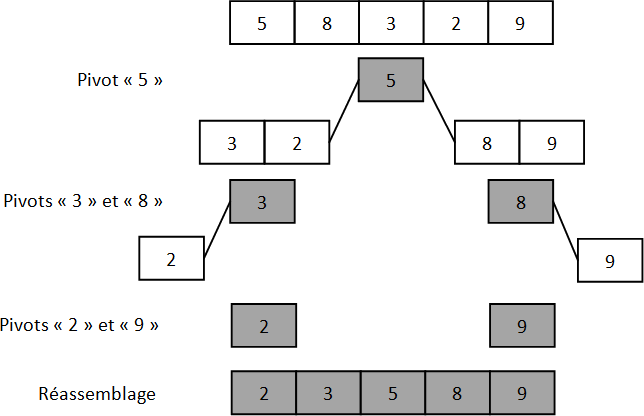
\includegraphics[width=\linewidth]{images/graphe_1}
\end{center}
\end{minipage}


Le « coût » temporel de l'algorithme de tri est principalement donné par des opérations de comparaison sur les éléments à trier. On raisonne donc sur le nombre de données à traiter pour l'analyse de la complexité de l'algorithme.

Dans le pire des cas, un des deux segments est vide à chaque appel de la fonction de tri. Cela arrive lorsque le tableau est déjà trié. Le nombre de données à traiter  pour le i\ieme appel, est $n - i + 1$.
Le nombre total pour n appels de fonction est donc $\dfrac{n(n+1)}{2}$. On peut aussi écrire une relation de récurrence du type $C(n) = C(n-1) + n - 1$
La complexité est donc de classe quadratique $C(n) = \mathcal{O}\left(n^2\right)$.

Dans le meilleur des cas, les deux segments sont de taille égale. Pour un nombre de données à traiter $n$, chacun des segments suivant a donc au plus $\dfrac{n-1}{2}$ éléments (on retire le pivot). On répète ainsi la segmentation des tableaux jusqu'à arriver au plus à un seul élément. 
On peut écrire une relation de récurrence du type $C(n) = 2 C\left(\dfrac{n - 1}{ 2} \right)  +  n - 1$.
 
La complexité est donc de classe quasi linéaire $C(n)=\mathcal{O}\left(n \ln(n)\right)$.

\begin{rem}
Certains algorithmes de tri rapide prennent pour « pivot » le dernier élément, la valeur moyenne du premier et du dernier, ou un positionnement aléatoire dans le tableau. Pour se placer dans le meilleur des cas pour chaque segment de tableau, il faut prendre pour pivot la valeur médiane du tableau de valeurs. Le problème est que cette recherche de pivot idéal a aussi un « coût ».
\end{rem}

On écrit tout d'abord l'algorithme effectuant la segmentation du tableau :
\begin{itemize}
\item le pivot (1\ier élément du tableau) est mis à sa place définitive;
\item pour des indices inférieurs, toutes les valeurs sont plus petites ou égales;
\item pour des indices supérieurs, toutes les valeurs sont plus grandes.
\end{itemize}

\begin{center}
\begin{tabular}{rc|c|c|c|c|c|}
\multicolumn{2}{c}{} & \multicolumn{1}{c}{$p=5$} & \multicolumn{1}{c}{$g$} & \multicolumn{2}{c}{}&  \multicolumn{1}{c}{$d$} \\
\cline{3-7}
$T[g]>p$ et $T[d]>p$&&\cellcolor{black!30}5 & \cellcolor{black!10}8 & 3 & 2 & \cellcolor{black!10}9 \\
\cline{3-7}
\multicolumn{2}{c}{} & 
\multicolumn{1}{c}{} & 
\multicolumn{1}{c}{$g$} & 
\multicolumn{1}{c}{}&  
\multicolumn{1}{c}{$d$}&  
\multicolumn{1}{c}{} \\
\cline{3-7}
$T[g]>p$ et $T[d]<p$, $d>g$ &&\cellcolor{black!30}5 & \cellcolor{black!10}8 & 3 & \cellcolor{black!10}2 & \cellcolor{black!10}9 \\
\cline{3-7}
\multicolumn{2}{c}{} & 
\multicolumn{1}{c}{} & 
\multicolumn{1}{c}{$g$} & 
\multicolumn{1}{c}{}&  
\multicolumn{1}{c}{$d$}&  
\multicolumn{1}{c}{} \\
\cline{3-7}
Échange de $T[g]$ et $T[d]$ &&\cellcolor{black!30}5 & \cellcolor{black!10}2 & 
3 & \cellcolor{black!10}8 & \cellcolor{black!10}9 \\
\cline{3-7}
\multicolumn{2}{c}{} & 
\multicolumn{1}{c}{} & 
\multicolumn{1}{c}{} & 
\multicolumn{1}{c}{$g=d$}&  
\multicolumn{1}{c}{}&  
\multicolumn{1}{c}{} \\
\cline{3-7}
$T[g]<p$ et $T[d]<p$, $g=d$ &&\cellcolor{black!30}5 & \cellcolor{black!10}2 & 
\cellcolor{black!10}3 & \cellcolor{black!10}8 & \cellcolor{black!10}9 \\
\cline{3-7}
\multicolumn{2}{c}{} & 
\multicolumn{1}{c}{} & 
\multicolumn{1}{c}{} & 
\multicolumn{1}{c}{$d$}&  
\multicolumn{1}{c}{$g$}&  
\multicolumn{1}{c}{} \\
\cline{3-7}
$g>d$ &&\cellcolor{black!30}5 & \cellcolor{black!10}2 & 
\cellcolor{black!10}3 & \cellcolor{black!10}8 & \cellcolor{black!10}9 \\
\cline{3-7}
\multicolumn{2}{c}{} & 
\multicolumn{1}{c}{} & 
\multicolumn{1}{c}{} & 
\multicolumn{1}{c}{}&  
\multicolumn{1}{c}{}&  
\multicolumn{1}{c}{} \\
\cline{3-7}
Échange de $p$ et $T[d]$ &&\cellcolor{black!10}3 & \cellcolor{black!10}2 & 
\cellcolor{black!30}5 & \cellcolor{black!10}8 & \cellcolor{black!10}9 \\
\cline{3-7}
\end{tabular}
\end{center}

Le pivot a sa place définitive. Les éléments à sa gauche sont plus petits ou égaux.
Les éléments à sa droite sont plus grands

\subsection{Algorithmes du tri rapide}

\begin{minipage}[c]{.48\linewidth}
\begin{pseudo}
~\\
\begin{tabular}{p{.98\textwidth}}
\hline
\textbf{Algorithme :} Tri Quicksort -- Segmentation\\
\hline
\textbf{Données :}
\begin{itemize}
\item \tsf{tab}, liste : une liste de nombres
\item \tsf{i,j}, entiers : indices de début et de fin de la segmentation à effectuer
\end{itemize}
\textbf{Résultats :} 
\begin{itemize}
\item \tsf{tab}, liste : la liste de nombre segmenté avec le pivot à sa place définitive
\item \tsf{k} entier : l'indice de la place du pivot
\end{itemize}
\\
\textbf{segmente}(\tsf{tab,i,j}) :\\
\hspace{.4cm} \tsf{g $\leftarrow$ i+1 }\\
\hspace{.4cm} \tsf{d $\leftarrow$ j}\\
\hspace{.4cm} \tsf{p $\leftarrow$ tab[i]}\\
\hspace{.4cm} \textbf{Tant que} \tsf{g $\leq$ d} \textbf{Faire} \\
\hspace{.8cm} \textbf{Tant que} \tsf{d$\geq$ 0} \textbf{et} \tsf{tab[d]>p} \textbf{Faire} \\
\hspace{1.2cm} \tsf{d $\leftarrow$ d-1}\\  
\hspace{.8cm} \textbf{Fin Tant que}  \\
\hspace{.8cm} \textbf{Tant que} \tsf{g$\leq$ j} \textbf{et} \tsf{tab[g]$\leq$p} \textbf{Faire} \\
\hspace{1.2cm} \tsf{g $\leftarrow$ g+1}\\  
\hspace{.8cm} \textbf{Fin Tant que}  \\
\hspace{.8cm} \textbf{Si} \tsf{g<d} \textbf{alors} \\
\hspace{1.2cm} \textbf{Échange(} \tsf{tab,g,d} \textbf{)} \\
\hspace{1.2cm} \tsf{d $\leftarrow$ d-1}\\  
\hspace{1.2cm} \tsf{g $\leftarrow$ g+1}\\  
\hspace{.8cm} \textbf{Fin Si} \\
\hspace{.4cm} \textbf{Fin Tant que}  \\
\hspace{.4cm} \tsf{k$\leftarrow$ d}  \\
\hspace{.4cm} \textbf{Échange(} \tsf{tab,i,d} \textbf{)} \\
\hspace{.4cm} \textbf{Retourner} \tsf{k}  \\
\hline
\end{tabular}
\end{pseudo}
\end{minipage}\hfill
\begin{minipage}[c]{.48\linewidth} 
\begin{py}
\begin{python}
def segmente(tab,i,j):
    """
    Segmentation d'un tableau par rapport à
    un pivot.
    Keyword arguments: 
    tab (list) -- liste de nombres
    i,j (int) -- indices de fin et de début de la 
    segmentation
    Retour :    
    tab (list) -- liste de nombres avec le pivot 
    à sa place définitive
    k (int) -- indice de la place du pivot
    """
    g =i+1
    d=j
    p=tab[i]
    while g<=d :
        while d>=0 and tab[d]>p:
            d=d-1
        while g<=j and tab[g]<=p:
            g=g+1
        if g<d :
            tab[g],tab[d]=tab[d],tab[g]
            d=d-1
            g=g+1
    k=d
    tab[i],tab[d]=tab[d],tab[i]
    return k
\end{python}
\end{py}
\end{minipage}

\begin{resultat}
Le nombre de comparaisons du type $T[d]>p$ et $T[g]\leq p$ est égal à $n-1$.
La complexité de cet algorithme est donc de classe linéaire : $C(n)=\mathcal{O}(n)$.
\end{resultat}

\begin{minipage}[c]{.48\linewidth}
\begin{pseudo}
\begin{tabular}{p{.9\linewidth}}
\hline
\textbf{Algorithme :} Tri Quicksort -- Tri rapide\\
\hline
\textbf{Données :}
\begin{itemize}
\item \tsf{tab}, liste : une liste de nombres
\item \tsf{i,j}, entiers : indices de début et de fin de la portion à trier
\end{itemize}
\textbf{Résultats :} 
\begin{itemize}
\item \tsf{tab}, liste : liste triée entre les indices \tsf{i} et \tsf{j}
\end{itemize}
\\
\textbf{tri\_quicksort}(\tsf{tab,i,j}) :\\
\hspace{.4cm} \textbf{Si} \tsf{g<d} \textbf{alors} \\
\hspace{.8cm} \tsf{k$\leftarrow$} \textbf{segmente(}\tsf{tab,i,j} \textbf{)} \\
\hspace{.8cm} \textbf{tri\_quicksort(}\tsf{tab,i,k-1} \textbf{)} \\
\hspace{.8cm} \textbf{tri\_quicksort(}\tsf{tab,k+1,j} \textbf{)} \\
\hspace{.4cm} \textbf{Fin Si} \\
\hline
\end{tabular}
\end{pseudo}
\end{minipage}\hfill
\begin{minipage}[c]{.48\linewidth} 
\begin{py}
\begin{python}
def tri_quicksort(tab,i,j):
    """
    Tri d'une liste par l'utilisation du 
    tri rapide (Quick sort).
    Keyword arguments: 
    tab (list) -- liste de nombres
    i,j (int) -- indices de fin et de 
    début de la zone de tri
    Retour :    
    tab (list) -- liste de nombres avec 
    le pivot à sa place définitive
    """
    if i<j :
        k = segmente(tab,i,j)
        tri_quicksort(tab,i,k-1)
        tri_quicksort(tab,k+1,j)
\end{python}
\end{py}
\end{minipage}


\begin{rem}
Cette méthode de tri est très efficace lorsque les données sont distinctes et non ordonnées. La complexité est alors globalement en $\mathcal{O}\left(n \ln(n))\right)$. Lorsque le nombre de données devient petit ($<15$) lors des appels récursifs de la fonction de tri, on peut avantageusement le remplacer par un tri par insertion dont la complexité est linéaire lorsque les données sont triées ou presque.
\end{rem}

\subsection{Tri rapide optimisé}


\begin{pseudo}
~\\

\begin{tabular}{p{.9\textwidth}}
\hline
\textbf{Algorithme :} Tri Quicksort -- Tri rapide optimisé\\
\hline
\textbf{Données :}
\begin{itemize}
\item \tsf{tab}, liste : une liste de nombres
\item \tsf{i,j}, entiers : indices de début et de fin de la portion de liste à trier
\end{itemize}
\textbf{Résultats :} 
\begin{itemize}
\item \tsf{tab}, liste : liste triée entre les indices \tsf{i} et \tsf{j}
\end{itemize}
\\
\textbf{tri\_quicksort\_optimized}(\tsf{tab,i,j}) :\\
\hspace{.4cm} \textbf{Si} \tsf{i<j} \textbf{alors} \\
\hspace{.8cm} \tsf{k$\leftarrow$} \textbf{segmente(}\tsf{tab,i,j} \textbf{)} \\
\hspace{.8cm} \textbf{Si} \tsf{k-i>15} \textbf{alors} \\
\hspace{1.2cm} \textbf{tri\_quicksort(}\tsf{tab,i,k-1} \textbf{)} \\
\hspace{.8cm} \textbf{Sinon} \\
\hspace{1.2cm} \textbf{tri\_insertion(}\tsf{tab,i,k-1} \textbf{)} \\
\hspace{.8cm} \textbf{Fin Si} \\
\hspace{.8cm} \textbf{Si} \tsf{j-k>15} \textbf{alors} \\
\hspace{1.2cm} \textbf{tri\_quicksort(}\tsf{tab,k+1,j} \textbf{)} \\
\hspace{.8cm} \textbf{Sinon} \\
\hspace{1.2cm} \textbf{tri\_insertion(}\tsf{tab,k+1,j} \textbf{)} \\
\hspace{.8cm} \textbf{Fin Si} \\
\hspace{.4cm} \textbf{Fin Si} \\
\hline
\end{tabular}
\end{pseudo}

\section{Le tri fusion}
\subsection{Méthode}
\begin{minipage}[c]{.48\linewidth}
La méthode de tri fusion pour un tableau de données est la suivante :
\begin{enumerate}
\item on coupe en deux parties à peu près égales les données à trier;
\item on trie les données de chaque partie par la méthode de tri fusion;
\item on fusionne les deux parties en interclassant les données.
\end{enumerate}

L'algorithme est donc récursif. Il fait partie des algorithmes « diviser pour régner ». La récursivité s'arrête car on finit par arriver à des listes composées d'un seul élément et le tri est alors trivial. 


\end{minipage} \hfill
\begin{minipage}[c]{.48\linewidth}
\begin{center}
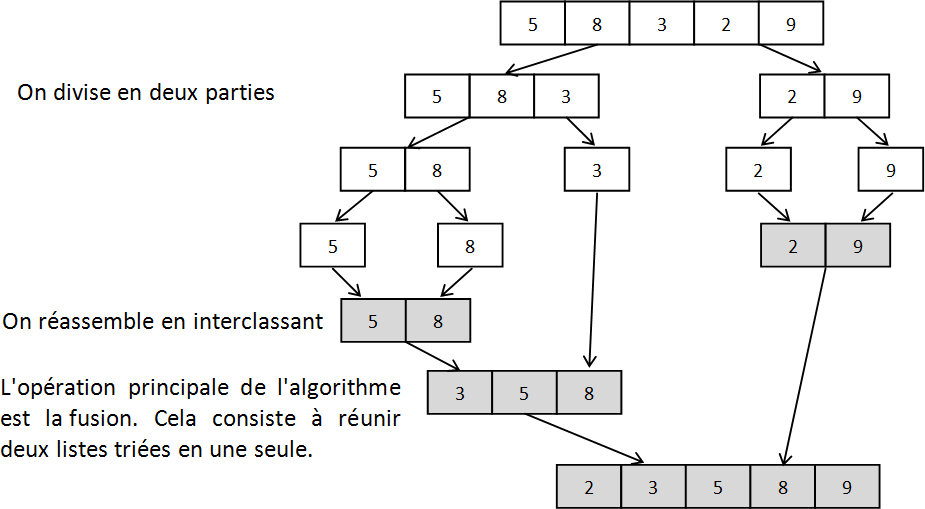
\includegraphics[width=\linewidth]{images/graphe_2}
\end{center}
\end{minipage}



\subsection{Algorithme de tri fusion}

\begin{minipage}[c]{.48\linewidth}
\begin{pseudo}
~\\
\begin{tabular}{p{.9\textwidth}}
\hline
\textbf{Algorithme :} Tri Fusion -- Fusion de deux listes\\
\hline
\textbf{Données :}
\begin{itemize}
\item \tsf{tab}, liste : une liste de nombres \tsf{tab[g:d]} avec \tsf{g} indice de la valeur de gauche, \tsf{d} indice de la valeur de droite
\item \tsf{m}, entier : indice tel que \tsf{$g\leq$m<d} et tel que les sous-tableaux \tsf{tab[g:m]} et \tsf{tab[m+1:d]} soient ordonnés
\end{itemize}
\textbf{Résultats :} 
\begin{itemize}
\item \tsf{tab}, liste : liste triée entre les indices \tsf{g} et \tsf{d}
\end{itemize}
\\
\textbf{fusion\_listes}(\tsf{tab,g,d,m}) :\\
\hspace{.4cm} \tsf{n1$\leftarrow$ m-g+1}\\
\hspace{.4cm} \tsf{n2$\leftarrow$ d-m}\\
\hspace{.4cm} \textbf{Initialiser tableau} \tsf{G}  \\
\hspace{.4cm} \textbf{Initialiser tableau} \tsf{D}  \\
\hspace{.4cm} \textbf{Pour} \tsf{i} \textbf{allant de} \tsf{1} \textbf{à} \tsf{n1} \textbf{faire}\\
\hspace{.8cm} \tsf{G[i] $ \leftarrow$ tab[g+i-1]}\\
\hspace{.4cm} \textbf{Fin Pour}\\
\hspace{.4cm} \textbf{Pour} \tsf{j} \textbf{allant de} \tsf{1} \textbf{à} \tsf{n2} \textbf{faire}\\
\hspace{.8cm} \tsf{D[j] $ \leftarrow$ tab[m+j]}\\
\hspace{.4cm} \tsf{Fin Pour}\\
\hspace{.4cm} \tsf{i $\leftarrow$ 1}\\
\hspace{.4cm} \tsf{j $\leftarrow$ 1}\\
\hspace{.4cm} \tsf{G[n1+1] $\leftarrow$ $+\infty$}\\
\hspace{.4cm} \tsf{D[n2+1] $\leftarrow$ $+\infty$}\\
\hspace{.4cm} \textbf{Pour} \tsf{k} \textbf{allant de} \tsf{g} \textbf{à} \tsf{d} \textbf{faire}\\
%\hspace{.8cm} \textbf{Si} \textsf{i$\leq$n1} \textbf{et} \textsf{G[i]$\leq$D[j]} \textbf{alors} \\
\hspace{.8cm} \textbf{Si}  \tsf{G[i]$\leq$D[j]} \textbf{alors} \\
\hspace{1.2cm} \tsf{tab[k]$\leftarrow$ G[i]} \\
\hspace{1.2cm} \tsf{i$\leftarrow$ i+1} \\
\hspace{.8cm} \textbf{Sinon} \\
%\hspace{1.2cm} \textbf{Si} \textsf{j$\leq$n2} \textbf{et} \textsf{G[i]>D[j]} \textbf{alors} \\
\hspace{1.2cm} \textbf{Si} \tsf{G[i]>D[j]} \textbf{alors} \\
\hspace{1.6cm} \tsf{tab[k]$\leftarrow$ D[j]} \\
\hspace{1.6cm} \tsf{j$\leftarrow$ j+1} \\
\hspace{1.2cm} \textbf{Fin Si} \\
\hspace{.8cm} \textbf{Fin Si} \\
\hspace{.4cm}  \textbf{Fin Pour}\\
\hline
\end{tabular}
\end{pseudo}
\end{minipage} \hfill
\begin{minipage}[c]{.48\linewidth}
\begin{py}
\begin{python}
def fusion_listes(tab,g,d,m):
    """
    Fusionne deux listes triées.
    Keyword arguments:
     * tab (list) -- liste : une liste de nombres 
        tab[g:d] avec g indice de la valeur de 
        gauche, d indice de la valeur de droite
     * g,d,m (int) -- entiers : indices tels que 
        g<=m<d et tel que les sous-tableaux
        tab[g:m] et tab[m+1:d] soient ordonnés
    Résultat :
     * tab (list) : liste triée entre les indices 
       g et d
    """
    n1 = m-g+1
    n2 = d-m
    G,D = [],[]
    for i in range (n1):
        G.append(tab[g+i])
    for j in range (n2):
        D.append(tab[m+j+1])
    i,j=0,0
    G.append(99999999999)
    D.append(99999999999)
    for k in range (g,d+1):
        if G[i]<=D[j]: # and i<=n1 
            tab[k]=G[i]
            i=i+1
        elif G[i]>D[j]: # and j<=n2
            tab[k]=D[j]
            j=j+1
\end{python}
\end{py}
\end{minipage} 

\begin{resultat}
Cet algorithme a une complexité en temps de classe linéaire : $C(n)=\mathcal{O}(n)$.
Par contre, il oblige à utiliser un espace supplémentaire égal à la taille du tableau original \texttt{tab}.
\end{resultat}

\begin{minipage}[c]{.48\linewidth}
\begin{pseudo}
~\\
\begin{tabular}{p{.9\textwidth}}
\hline
\textbf{Algorithme :} Tri Fusion \\
\hline
Algorithme récursif du table de tri. \\
\textbf{Données :}
\begin{itemize}
\item \tsf{tab}, liste : une liste de nombres non triés \tsf{tab[g:d]} 
\item \tsf{g,d}, entiers : indices de début et de fin de la liste
\end{itemize}
\textbf{Résultats :} 
\begin{itemize}
\item \tsf{tab}, liste : liste triée entre les indices \tsf{g} et \tsf{d}
\end{itemize}
\\
\textbf{tri\_fusion}(\tsf{tab,g,d}) :\\
\hspace{.4cm} \textbf{Si} \tsf{g<d}  \textbf{alors} \\
\hspace{.8cm} \tsf{m $\leftarrow$ (g+d)} \textbf{div} 2\\
\hspace{.8cm} \textbf{tri\_fusion}(tab,g,m) \\
\hspace{.8cm} \textbf{tri\_fusion}(tab,m+1,d) \\
\hspace{.8cm} \textbf{fusion\_listes}(tab,g,d,m) \\
\hspace{.4cm}  \textbf{Fin Si}\\
\hline
\end{tabular}
\end{pseudo}
\end{minipage}\hfill
\begin{minipage}[c]{.48\linewidth}
\begin{py}
\begin{python}        
def tri_fusion(tab,g,d):
    """
    Tri d'une liste par la métode du tri fusion
    Keyword arguments:
    tab (list) -- liste : une liste de nombres non 
      triés tab[g:d]
    g,d (int) -- entiers : indices de début et 
      de fin de liste si on veut trier
      tout le tableau g=0, d=len(tab)-1
    Résultat :
    tab (list) : liste triée entre les indices 
      g et d
    """
    if g<d:
        m=(g+d)//2
        tri_fusion(tab,g,m)
        tri_fusion(tab,m+1,d)
        fusion_listes(tab,g,d,m)
\end{python}
\end{py}
\end{minipage}

Si l'on s'intéresse au nombre de données à traiter à chaque appel de fonction, la relation de récurrence est du type :
$C(n) = 2 C\left(\dfrac{n}{2}\right)  +  n$.
La méthode de tri fusion a donc une efficacité temporelle comparable au tri rapide en $\mathcal{O}\left(n \ln(n)\right)$. Par contre, elle n'opère pas en place : une zone temporaire de données supplémentaire de taille égale à celle de l'entrée est nécessaire. Des versions plus complexes peuvent être effectuées sur place mais sont moins rapides.










\section{Synthèse}

\begin{center}
\begin{tabular}{|c|c|c|c|}
\hline
& Tri par insertion$^1$ & Tri rapide & Tri fusion \\
\hline 
{Pire des cas} &  Liste triée& Liste triée$^2$ & \\ 
&  $ C(n)=\mathcal{O}\left(n^2 \right)$ & $ C(n)=\mathcal{O}\left(n^2 \right)$ & $ C(n)=\mathcal{O}\left(n \log n\right)$ \\ \hline
Cas moyen & $ C(n)=\mathcal{O}\left(n^2 \right)$ &$ C(n)=\mathcal{O}\left(n \log n\right)$  & $ C(n)=\mathcal{O}\left(n \log n\right)$ \\ \hline
Meilleur des cas  & Liste triée & Liste triée$^3$ & \\ 
  & $ C(n)=\mathcal{O}\left(n \right)$ & $ C(n)=\mathcal{O}\left(n \right)$ & $ C(n)=\mathcal{O}\left(n \log n\right)$ \\ \hline
\end{tabular}
\end{center}

\footnotesize{1 : dépend de la méthode de tri.}

\footnotesize{2 : lorsque le pivot est la première valeur des listes.}

\footnotesize{3 : lorsque le pivot est pris au milieu des listes.}
\begin{thebibliography}{2}
\bibitem{1}{Patrick Beynet, \textit{Supports de cours de TSI 2}, Lycée Rouvière, Toulon.}

\end{thebibliography}
\end{document}

